\documentclass[10pt, a4paper]{article}
% \usepackage[english]{babel}
\usepackage[brazilian]{babel}
\usepackage[utf8]{inputenc}
% \usepackage[T1]{fontenc}

% matlab code
% \usepackage{matlab-prettifier}
\usepackage[numbered,framed]{matlab-prettifier}
\renewcommand{\lstlistingname}{Anexo} % Listing->Code
\let\ph\mlplaceholder % shorter macro
\definecolor{codegreen}{rgb}{0,0.6,0}
\definecolor{codegray}{rgb}{0.5,0.5,0.5}
\definecolor{codepurple}{rgb}{0.58,0,0.82}
\definecolor{backcolour}{rgb}{0.95,0.95,0.92}
\lstdefinestyle{myStyle}{
    language=Matlab,
    breaklines=true,
    frame=single,
    numbers=none,
    basicstyle=\ttfamily\footnotesize,
%     basicstyle=\footnotesize\ttfamily,
    keywordstyle=\bfseries\color{magenta},
    commentstyle=\color{codegreen},
    identifierstyle=\color{blue},
    backgroundcolor=\color{backcolour},
    stringstyle=\color{codepurple},
}
\usepackage{adjustbox}
\usepackage[skip=10pt]{parskip}
% \usepackage{setspace}

% For subfigure use
\usepackage[font=small,labelfont=bf]{caption}
\usepackage{subcaption}

% Set page size and margins
% Replace `letterpaper' with`a4paper' for UK/EU standard size
\usepackage[a4paper,top=2cm,bottom=2cm,left=2cm,right=2cm,marginparwidth=2cm]{geometry}

% tabelas
\usepackage{array}
\usepackage{tabularx}
\usepackage{booktabs}
\usepackage{multirow}

\usepackage{float}

% Useful packages
\usepackage{amsmath}

\usepackage{graphicx}
\graphicspath{{figures/}} %Setting the graphicspath
\usepackage[colorlinks=true, allcolors=blue]{hyperref}

% \title{PUC-RJ Pontif\'icia Universidade Cat\'olica do Rio de Janeiro \\ MEC 2403 - Otimiza\c c\~ao e Algoritmos para Engenharia Mec\^anica \\ Trabalho 02 - Otimiza\c c\~ao com Restri\c c\~oes  \\
% \large Professor: Ivan Menezes}

% \author{Felipe da Costa Pereira - mat. 2212376 \\ {\tt felipecostapereira@gmail.com}}

\begin{document}

\begin{titlepage}
      \begin{center}
          \vspace*{1cm}

          \Huge
          \textbf{Trabalho 02 \\ Otimiza\c c\~ao com Restri\c c\~oes}

          \vspace{0.5cm}
          \LARGE
          MEC 2403 - Otimiza\c c\~ao e Algoritmos para Engenharia Mec\^anica

          \vspace{1.5cm}

          \textbf{Felipe da Costa Pereira \\ {\tt felipecostapereira@gmail.com}}

          \vfill
          Professor: Ivan Menezes

          \vspace{0.8cm}

          
\includegraphics[width=0.2\textwidth]{puc.jpg}

          \Large
          Departamento de Engenharia Mec\^anica\\
          PUC-RJ Pontif\'icia Universidade Cat\'olica do Rio de Janeiro\\
          Novembro, 2022

      \end{center}
  \end{titlepage}

\section{Introdu\c c\~ao}

Otimiza\c c\~ao com restri\c c\~ao \'e o processo que minimiza uma fun\c c\~ao objetivo em rela\c c\~ao a algumas vari\'aveis em presen\c ca de restri\c c\~oes aos valores dessas vari\'aveis.

\[
\begin{cases}
      \begin{aligned}
      \text{Minimizar }  & f(\vec{x})\\
      \text{Sujeito a: } & h_k(\vec{x})=0,            \text{$k=1...m$}\\
                        & c_l(\vec{x})\leq 0,        \text{$l=1...p$}\\
                        & x_i^L \leq x_i \leq x_i^U, \text{$i=1...n$}
      \end{aligned}
\end{cases}
\]

As equa\c c\~oes $h_k$ e $c_l$ representam as restri\c c\~oes de igualdade e desigualdade, respectivamente. J\'a os valores $x_i^L$ e $x_i^U$ representam os limites laterais da vari\'avel $x_i$.

Para solu\c c\~ao dos problemas desse trabalho, que consiste na minimiza\c c\~ao de algumas fun\c c\~oes sob certas restri\c c\~oes, iremos utilizar os m\'etodos indiretos, s\~ao eles o m\'etodo de penalidade e o de barreira.

\section{Objetivos}

Os principais objetivos deste trabalho s\~ao:
\begin{itemize}
      \item Implementar numericamente os algoritmos indiretos de otimiza\c c\~ao com restri\c c\~oes: penalidade e barreira.
      \item Avaliar a influ\^encia dos par\^ametros dos algoritmos nas m\'etricas de converg\^encia e comparar essas \'ulltimas com os valores esperados da teoria.
      \item Aplicar os algoritmos implementados na solu\c c\~ao do problema de OCR em dois casos: uma fun\c c\~ao polinomial de ordem 4 e uma fun\c c\~ao que representa um problema de engenharia (minimiza\c c\~ao do peso de uma treli\c ca de duas barras e cujas restri\c c\~oes est\~ao associadas a valores m\'aximos de tens\~ao nas barras das treli\c cas que n\~ao podem ser maiores do que as tens\~oes cr\'itica de Euler e de escoamento do material)
\end{itemize}

As fun\c c\~oes a serem minimizadas neste trabalho e as respectivas restri\c c\~oes s\~ao:

\textbf{Problema 01:}
\[
      \begin{cases}
            \begin{aligned}
            \text{Minimizar:  }   & f(x_1, x_2) = (x_1-2)^4 + (x_1-2x_2)^2 \\
            \text{Sujeito a:  }   & x_1^2 - x_2 \leq 0\\
            \end{aligned}
      \end{cases}
\]
Partindo do ponto $x^0=\{3,2\}$ para o m\'etodo da penalidade e do ponto $x^0=\{0,1\}$ para o m\'etodo de barreira.

\textbf{Problema 02:}
\[
      \begin{cases}
            \begin{aligned}
            \text{Minimizar:  }     & f(d, H) = 2\rho \pi t d \sqrt{H^2+B^2}\\
            \text{Sujeito a:  }     & \frac{P \sqrt{H^2+B^2}}{\pi t d H} \leq \sigma_y \text{ e } \frac{P \sqrt{H^2+B^2}}{\pi t d H} \leq \frac{\pi^2 E (d^2+t^2)}{8(H^2+B^2)}\\
            \end{aligned}
      \end{cases}
\]
\small
\[
\text{Onde:} \begin{cases}
      \text{d: di\^ametro m\'edio da se\c c\~ao transversal}\\
      \text{t: espessura da se\c c\~ao transversal}\\
      \text{E: m\'odulo de elasticidade do material}\\
      \text{$\rho$: peso espec\'ifico do material}
\end{cases}
\]
\normalsize
Partindo do ponto $x^0=\{1,15\}$ para o m\'etodo da penalidade e do ponto $x^0=\{4,25\}$ para o m\'etodo de barreira.


\section{M\'etodos Indiretos em OCR}

Segundo \cite{apostila}, as primeiras tentativas de se resolver o problema de otimiza\c c\~ao com restri\c c\~oes (OCR) foram feitas utilizando-se os m\'etodos indiretos, nomeadamente, os m\'etodos de penalidade e os de barreira. Esses m\'etodos resolvem problemas de OCR por meio de uma sequ\^encia de solu\c c\~oes de problemas de OSR. Para que isso seja poss\'ivel, as restri\c c\~oesoes dos problemas de OCR s\~ao incorporadas \`a fun\c c\~ao objetivo criando-se as chamadas fun\c c\~oes de penalidade (e de barreira) que s\~ao usadas nos problemas de OSR. A id\'eia da fun\c c\~ao de penalidade (e de barreira) \'e criar um alto custo pela viola\c c\~ao das restri\c c\~oes o que for\c ca a solu\c c\~ao a atender as restri\c c\~oes. Os m\'etodos indiretos apresentam, em geral, dificuldades computacionais e por isso v\^em sendo substitu\'idos pelos m\'etodos diretos. Eles t\^em, no entanto, o atrativo de serem m\'etodos simples de se resolver problemas de OCR e apresentam uma import\^ancia hist\'orica no desenvolvimento de m\'etodos de programa\c c\~ao matem\'atica.

A pseudo-fun\c c\~ao objetivo \'e dada por (\cite{ppt}):

\begin{equation}
      \phi (\vec{x}, r) = f(\vec{x}) + r \times p(\vec{x})
\end{equation}

\small
$$
\text{Onde:} \begin{cases}
      \text{r: escalar que define a magnitude da penaliza\c c\~ao}\\
      \text{$p(\vec{x})$: fun\c c\~ao penalidade}\\
      \text{$f(\vec{x})$: fun\c c\~ao objetivo original}\\
      \text{$\phi (\vec{x}, r)$: pseudo-fun\c c\~ao objetvo}
\end{cases}
$$
\normalsize

Para evitar problemas num\'ericos de mal condicionamento, a penalidade $r$ \'e introduzida de forma gradual, iniciando-se moderada e tendo seu valor incrementado a medida em que o processo de otimiza\c c\~ao se desenvolve. Dessa forma a solu\c c\~ao de um Problema de OCR se torna uma sequ\^encia de Problemas de OSR (\cite{ppt}).

\subsection{M\'etodo da Penalidade}

O m\'etodo de penalidade para restri\c c\~oes de desigualdade \'e tamb\'em chamado de m\'etodo exterior porque ele tem a caracter\'istica de se aproximar da solu\c c\~ao pela regi\~ao n\~ao vi\'avel, ou seja, violando as restri\c c\~oes. Essa caracter\'istica n\~ao \'e vantajosa porque, se o processo iterativo for interrompido por qualquer raz\~ao, como mal condicionamento num\'erico, a solu\c c\~ao obtida n\~ao \'e uma solu\c c\~ao vi\'avel do problema (\cite{apostila}).

\begin{equation} \label{eqPen}
      \phi (\vec{x}, r_p) = f(\vec{x}) + \frac{1}{2} r_p \sum_{k=1}^{m} h_k^2(\vec{x}) + \frac{1}{2} r_p \sum_{l=1}^{p} \{max[0,c_l(\vec{x})]^2
\end{equation}

Podemos observar pela eq. \ref{eqPen} que caso a restri\c c\~ao seja atendida (ponto na regi\~ao vi\'avel), $c_l \leq 0$, logo, a fun\c c\~ao $\phi$ n\~ao possui o termo da fun\c c\~ao de penalidade e enconrtrar o m\'inimo de $\phi$ equivale a encontrar o m\'inimo de $f$. Assim, o ponto em quest\~ao ir\'a para a regi\~ao n\~ao vi\'avel, por onde converge o algoritmo da penalidade.

O passo a passo do m\'etodo da penalidade \'e descrito na figura \ref{fig:algoritmoPenalidade}

\begin{figure}[H]
      \centering
      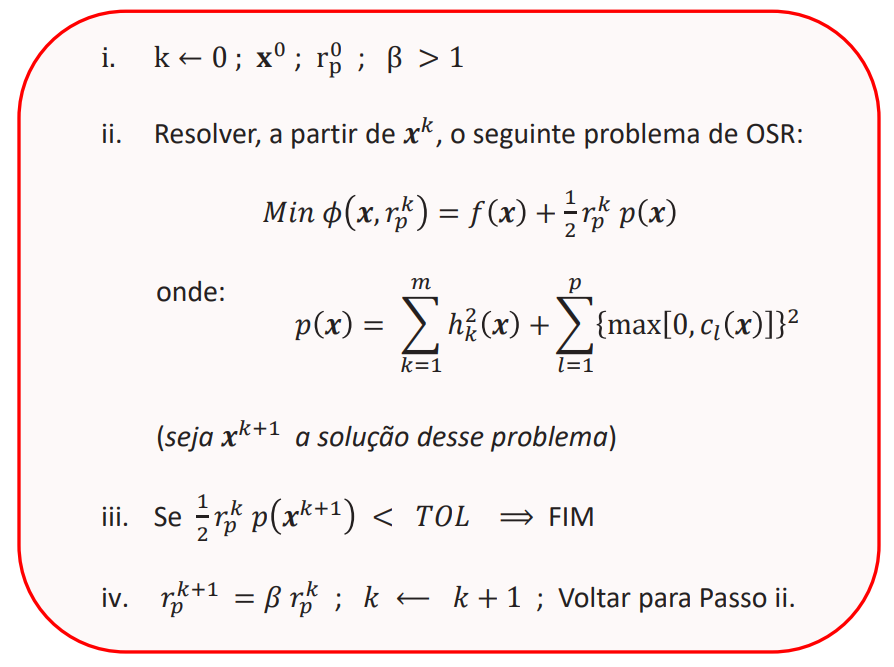
\includegraphics[width=.6\textwidth]{algoritmoPenalidade.PNG}
      \caption{Principais passos do m\'etodo da penalidade (\cite{ppt})}
      \label{fig:algoritmoPenalidade}
\end{figure}

\subsection{M\'etodo da Barreira}

No m\'etodo da barreira (ou m\'etodo interior), a converg\^encia se d\'a do interior da regi\~ao das solu\c c\~oes vi\'aveis para o contorno dela. Essa caracter\'istica torna a solu\c c\~ao em cada itera\c c\~ao do processo uma solu\c c\~ao vi\'avel, o que \'e interessante. O m\'etodo usa a denomina\c c\~ao barreira porque a fun\c c\~ao de barreira se torna infinita no contorno da regi\~ao vi\'avel.

\begin{equation} \label{eqBarr}
      \phi (\vec{x}, r_p) = f(\vec{x}) + r_b \sum_{k=1}^{m} h_k^2(\vec{x}) + r_b \sum_{l=1}^{p} - \frac{1}{c_l(\vec{x})}
\end{equation}

Como, no caso da barreira, a solu\c c\~ao converge pela regi\~ao vi\'avel, $c_l \leq 0$ e, portanto, existe um sinal negativo na eq. \ref{eqBarr} para tornar a pseudo-fun\c c\~ao objetivo $\phi$ postiva e, consequentemente, permitir sua minimiza\c c\~ao, caso contr\'ario esta iria para $-\infty$, j\'a que $c_l$ tende a se aproximar de zero \`a medida que as itera\c c\~oes avan\c cam.

O passo a passo do m\'etodo da barreira \'e descrito na figura \ref{fig:algoritmoBarreira}

\begin{figure}[H]
      \centering
      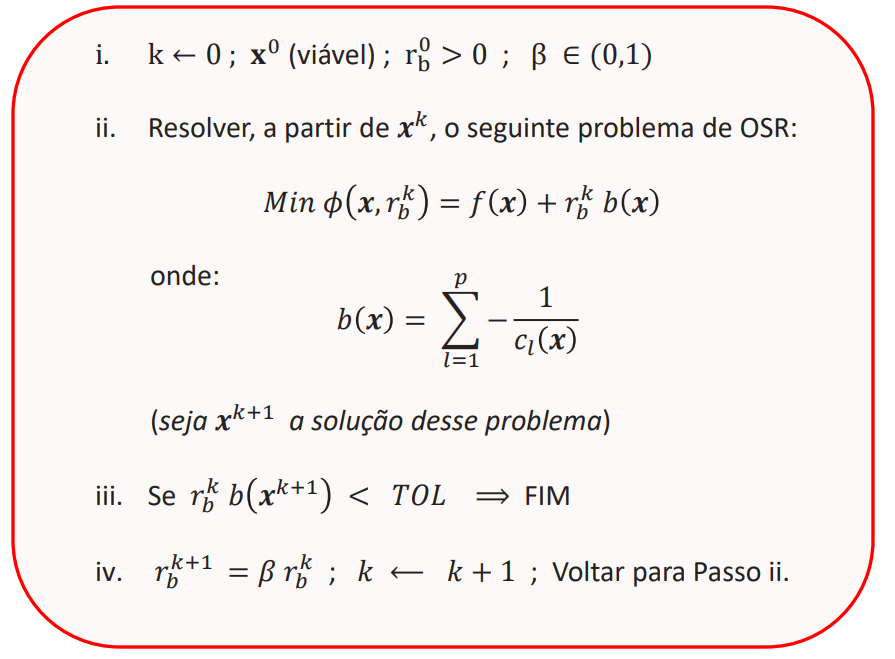
\includegraphics[width=.6\textwidth]{algoritmoBarreira.PNG}
      \caption{Principais passos do m\'etodo da barreira (\cite{ppt})}
      \label{fig:algoritmoBarreira}
\end{figure}

\section{Resultados}

Visando a converg\^encia de todos os m\'etodos, foram testados alguns valores dos par\^ametros dos algoritmos. A melhor combina\c c\~ao dos par\^ametros, para as fun\c c\~oes dos problemas 1 e 2 em termos de converg\~encia dos algoritmos est\'a listada na tabela \ref{table:params}.

O processo de busca linear implementado para solu\c c\~ao do problema de OSR possui inefici\^encias e imperfei\c c\~oes, principalmente no caso das fun\c c\~oes-objetivo serem mais complexas quando associadas aos termos de penalidade, conforme \'e o caso das pseudo-fun\c c\~os objetivo associadas aos casos de OCR. Este fato levou a dificuldades na converg\^encia dos algortimos, em geral.

Foram testados valores de toler\^ancias menores, na faixa de $10^{-6}$, e $d\alpha$ (passo da busca linear) maiores. Nesses casos, os algortimos at\'e convergiam, por\'em em temos muito longos, o que prejudicou a possibilidade de testes e execu\c c\~ao do trabalho. Dessa forma, o programa implementado para a solu\c c\~ao dos problemas de OCR utilizou os valores da tabela \ref{table:params}.

\small
$$
\text{Par\^ametros:} \begin{cases}
      \text{$d\alpha$:  tamanho do passo do algoritmo do passo constante}\\
      \text{TOL(BL):    toler\^ancia associada ao algoritmo da Busca Linear no problema de OSR}\\
      \text{TOL(OCR):   toler\^ancia utilizada para verificar a converg\^encia dos algortimos de OCR}\\
      \text{TOL(SA):    toler\^ancia associada ao algoritmo da Se\c c\~ao \'Aurea no problema de OSR}\\
      \text{$\beta$:    multiplicados do termo de penaliza\c c\~ao $r$ da pseudo-fun\c c\~ao objetivo do algoritmo de OCR}
\end{cases}
$$
\normalsize

\begin{table}[H]
      \small
      \centering
      \caption{Melhores par\^ametros para converg\^encia dos algoritmos}
      \begin{tabular}{c|c|c|c|c|c|c|c}
            Problema & M\'etodo & Algoritmo & $d\alpha$ & TOL(BL) & TOL(OCR) & TOL(SA) & $\beta$ \\
            \hline
            \multirow{6}{*}{01} & \multirow{6}{*}{Penalidade} & Univariante       & 0.002 & $10^{-4}$ & $10^{-4}$ & $10^{-6}$ & 5   \\
                                                            & & Powell            & 0.002 & $10^{-4}$ & $10^{-4}$ & $10^{-5}$ & 10  \\
                                                            & & Steepest Descent  & 0.002 & $10^{-4}$ & $10^{-4}$ & $10^{-9}$ & 5   \\
                                                            & & Flecher-Reeves    & 0.001 & $10^{-4}$ & $10^{-4}$ & $10^{-7}$ & 5   \\
                                                            & & Newton-Raphson    & 0.05  & $10^{-4}$ & $10^{-4}$ & $10^{-7}$ & 20  \\
                                                            & & BFGS              & 0.04  & $10^{-5}$ & $10^{-5}$ & $10^{-8}$ & 10  \\
            \hline
            \multirow{6}{*}{01} & \multirow{6}{*}{Barreira} & Univariante         & 0.0002 & $10^{-4}$ & $10^{-4}$ & $10^{-8}$ & 0.05 \\
                                                            & & Powell            & 0.0002 & $10^{-4}$ & $10^{-4}$ & $10^{-5}$ & 0.2  \\
                                                            & & Steepest Descent  & 0.0002 & $10^{-4}$ & $10^{-4}$ & $10^{-7}$ & 0.05 \\
                                                            & & Flecher-Reeves    & 0.0002 & $10^{-4}$ & $10^{-4}$ & $10^{-7}$ & 0.05 \\
                                                            & & Newton-Raphson    & 0.002  & $10^{-6}$ & $10^{-6}$ & $10^{-7}$ & 0.05 \\
                                                            & & BFGS              & 0.0002 & $10^{-4}$ & $10^{-4}$ & $10^{-5}$ & 0.05 \\
            \hline
            \multirow{6}{*}{02} & \multirow{6}{*}{Penalidade} & Univariante       & 0.005  & $10^{-6}$ & $10^{-6}$ & $10^{-7}$ & 10 \\
                                                            & & Powell            & 0.005  & $10^{-6}$ & $10^{-6}$ & $10^{-5}$ & 50 \\
                                                            & & Steepest Descent  & 0.0001 & $10^{-3}$ & $10^{-4}$ & $10^{-7}$ & 10 \\
                                                            & & Flecher-Reeves    & 0.0001 & $10^{-3}$ & $10^{-4}$ & $10^{-7}$ & 10 \\
                                                            & & Newton-Raphson    & 0.0002 & $10^{-5}$ & $10^{-6}$ & $10^{-7}$ & 10 \\
                                                            & & BFGS              & 0.0002 & $10^{-3}$ & $10^{-4}$ & $10^{-7}$ & 10 \\
            \hline
            \multirow{6}{*}{02} & \multirow{6}{*}{Barreira} & Univariante         & 0.0001  & $10^{-4}$ & $10^{-4}$ & $10^{-9}$  & 0.12   \\
                                                            & & Powell            & 0.0001  & $10^{-4}$ & $10^{-4}$ & $10^{-10}$ & 0.09   \\
                                                            & & Steepest Descent  & 0.00002 & $10^{-4}$ & $10^{-4}$ & $10^{-9}$  & 0.005  \\
                                                            & & Flecher-Reeves    & 0.00002 & $10^{-4}$ & $10^{-4}$ & $10^{-7}$  & 0.008  \\
                                                            & & Newton-Raphson    & 0.001   & $10^{-6}$ & $10^{-6}$ & $10^{-6}$  & 0.01   \\
                                                            & & BFGS              & 0.0002  & $10^{-5}$ & $10^{-4}$ & $10^{-8}$  & 0.0006 \\
            \hline
      \end{tabular}
      \label{table:params}
\end{table}


A tabela \ref{table:results} abaixo ilustra os resultados encontrados para a implementa\c c\~ao dos m\'etodos de penalidade e barreira para as fun\c c\~oes e restri\c c\~oes dos problemas 01 e 02. Al\'em dos pontos de m\'inimo encontrados, a tabela apresenta tamb\'em o n\'umero de passos para a converg\^encia e o tempo de execu\c c\~ao. Estes dois \'ultimos representam quantas vezes foi chamado o script de solu\c c\~ao do problema de OSR e quanto tempo computacional foi consumido no total de itera\c c\~oes, respectivamente.

\begin{table}[H]
      \small
      \centering
      \caption{Resultados}
      \begin{tabular}{c|c|c|c|c|c|c}
            Problema & M\'etodo, $x^0$  & Algoritmo & $x^{min}$ & passos & $\Delta t$(ms) \\
            \hline
            \multirow{6}{*}{01} & \multirow{6}{*}{Penalidade, $x^0=\{3,2\}$} & Univariante       & $\{0.9446,0.8921\}$ & 8 & 55.3  \\
                                                            & & Powell            & $\{0.9456,0.8941\}$ & 6 & 198.4 \\
                                                            & & Steepest Descent  & $\{0.9456,0.8941\}$ & 8 & 20.8  \\
                                                            & & Flecher-Reeves    & $\{0.9456,0.8941\}$ & 8 & 5.9   \\
                                                            & & Newton-Raphson    & $\{0.9456,0.8941\}$ & 5 & 3.9   \\
                                                            & & BFGS              & $\{0.9456,0.8941\}$ & 7 & 2.4   \\
            \hline
            \multirow{6}{*}{01} & \multirow{6}{*}{Barreira, $x^0=\{0,1\}$} & Univariante         & $\{0.9467,0.8969\}$ & 6  & 78.0   \\
                                                            & & Powell            & $\{0.9453,0.8944\}$ & 11 & 8615.5 \\
                                                            & & Steepest Descent  & $\{0.9456,0.8948\}$ & 6  & 797.9  \\
                                                            & & Flecher-Reeves    & $\{0.9454,0.8944\}$ & 6  & 297.1  \\
                                                            & & Newton-Raphson    & $\{0.9456,0.8941\}$ & 10 & 124.0  \\
                                                            & & BFGS              & $\{0.9454,0.8944\}$ & 6  & 239.1  \\
            \hline
            \multirow{6}{*}{02} & \multirow{6}{*}{Penalidade, $x^0=\{1,15\}$} & Univariante       & $\{1.8784,20.2363\}$ & 15 & 144.3   \\
                                                            & & Powell            & $\{1.8783,20.2365\}$ & 8  & 247.3   \\
                                                            & & Steepest Descent  & $\{1.8784,20.2357\}$ & 14 & 5302.9  \\
                                                            & & Flecher-Reeves    & $\{1.8783,20.2350\}$ & 12 & 1920.4  \\
                                                            & & Newton-Raphson    & $\{1.8783,20.2365\}$ & 15 & 528.7   \\
                                                            & & BFGS              & $\{1.8783,20.2363\}$ & 13 & 6433.7  \\
            \hline
            \multirow{6}{*}{02} & \multirow{6}{*}{Barreira, $x^0=\{4,25\}$} & Univariante         & $\{1.8785,20.2389\}$ & 15 & 13461.8 \\
                                                            & & Powell            & $\{1.8785,20.2396\}$ & 13 & 11053.0 \\
                                                            & & Steepest Descent  & $\{1.8793,20.8871\}$ & 5  & 9248.0  \\
                                                            & & Flecher-Reeves    & $\{1.8855,20.3466\}$ & 5  & 3708.0  \\
                                                            & & Newton-Raphson    & $\{1.8784,20.2367\}$ & 8  & 225.5   \\
                                                            & & BFGS              & $\{1.8971,20.5055\}$ & 3  & 1675.9  \\
            \hline
      \end{tabular}
      \label{table:results}
\end{table}

\newpage

Conforme citado anteriormente, a utliza\c c\~ao de m\'etodos indiretos em OCR consiste na incorpora\c c\~ao das restri\c c\~oes na fun\c c\~ao objetivo a ser minimizada, sendo os termos associados \`as restri\c c\~oes penalizados gradualmente.

Nas figuras a seguir, para cada passo dos algoritmos de penalidade ou barreira, ilustra-se as curvas de n\'ivel da pseudo-fun\c c\~ao objetivo $\phi(x_1, x_2)$, onde se pode evidenciar a forma que esta vai tomando a cada passo do m\'etodo, a partir da incorpora\c c\~ao e penaliza\c c\~ao dos termos de restri\c c\~ao.

Sobrepostos \`as curvas de n\'ivel de $\phi(x_1, x_2)$, para cada passo $k=1....n$ ilustra-se o conjunto de pontos $\{x^0, x^1, ... , x^k\}$ (solu\c c\~oes do problema de OSR) at\'e o passo atual.

%%%%%%%%%%%%%%%%%%%%%%%%%%%
% PROBLEMA 01
%%%%%%%%%%%%%%%%%%%%%%%%%%%

As figuras a seguir ilustram as curvas da solu\c c\~ao de OCR para a fun\c c\~ao a as restri\c c\~oes do problema 1

Na figura \ref{fig:fig01} podemos ver a regi\~ao vi\'avel (acima da curva vermelha) e a converg\^encia do algoritmo pelo algortimo de Powell de OSR, assim como a deforma\c c\~ao de $\phi(x_1,x_2)$ a partir do ponto $x^0=\{3,2\}$. Nota-se tamb\'em a converg\^encia do algoritmo pela regi\~ao n\~ao vi\'avel (abaixo da curva vermelha).

\begin{figure}[H]
      \centering
      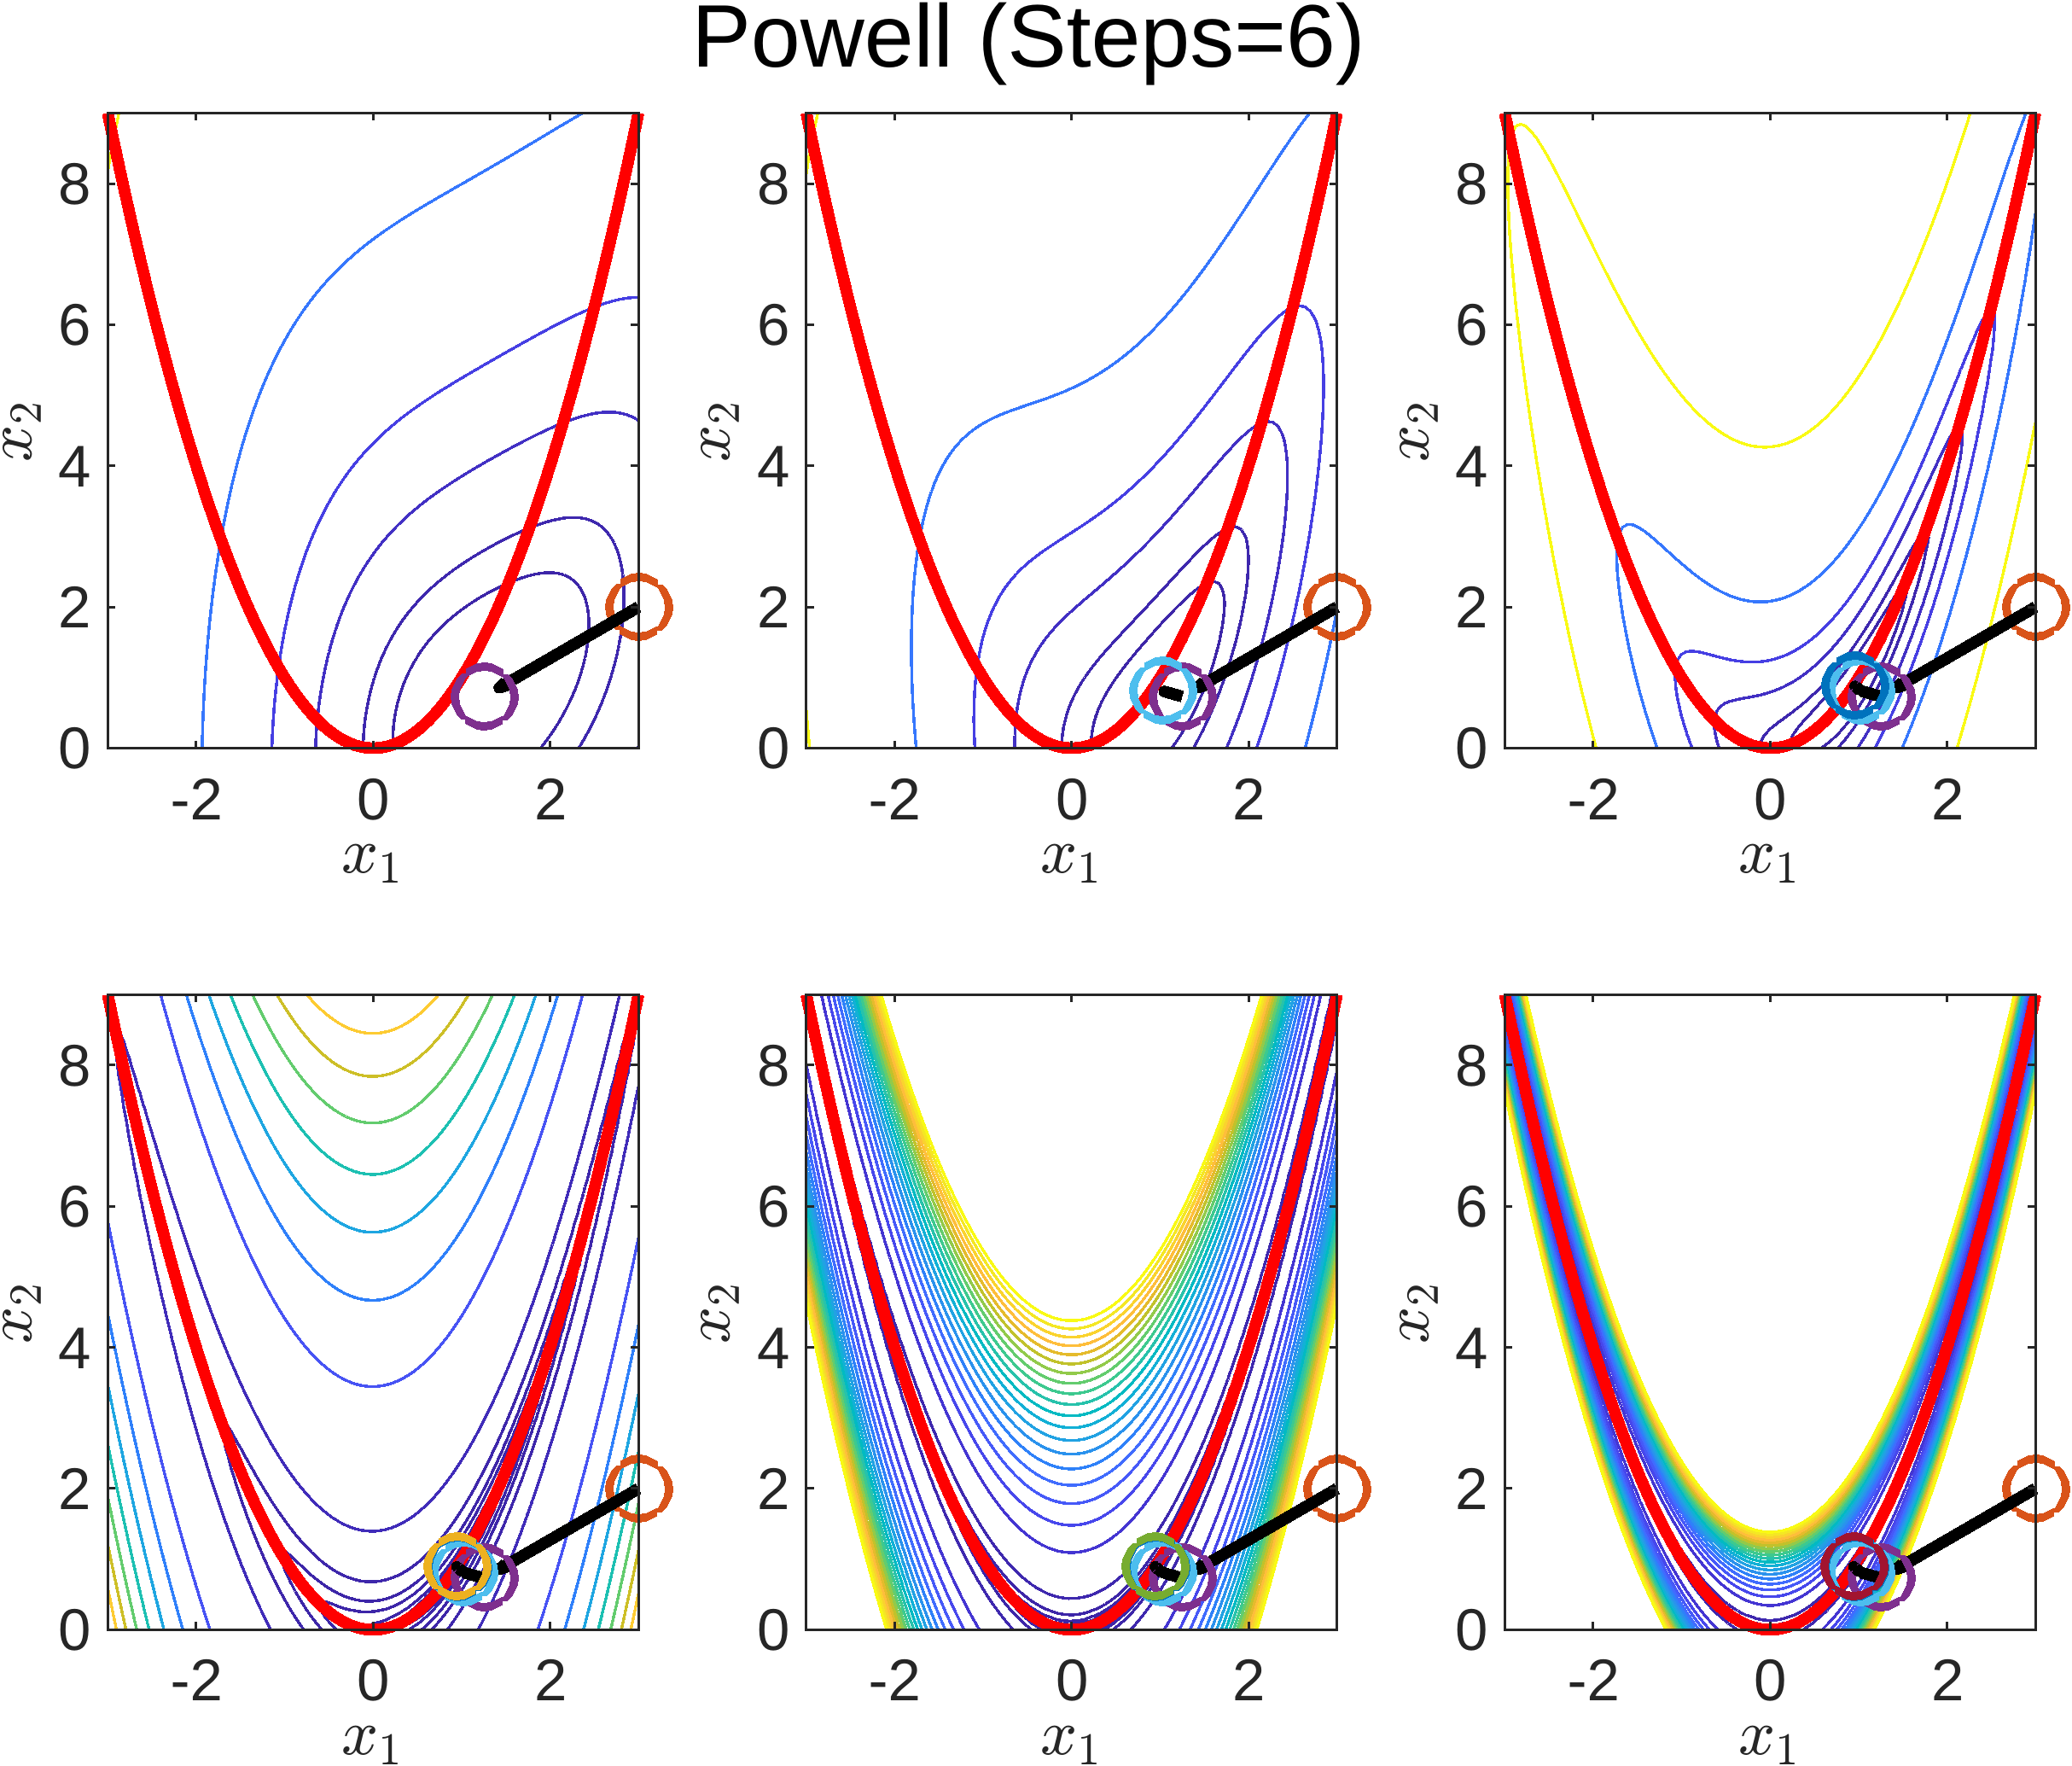
\includegraphics[width=0.65\textwidth]{fig01_P01_PEN_X1_POW.png}
      \caption{OCR do problema 01 pelo m\'etodo da penalidade, a partir do ponto $x^0=\{3,2\}$ - Algoritmo de Powell}
      \label{fig:fig01}
\end{figure}

Para avaliar a robustez dos algoritmos, selecionamos um novo ponto $x^0=\{0,4\}$, desta vez dentro da regi\~ao vi\'avel, uma vez que, diferente do m\'etodo de barreira, n\~ao \'e uma exig\^encia do algortimo que o ponto inicial seja um ponto vi\'avel. Nota-se que logo no primeiro passo, a solu\c c\~ao de OSR de $\phi$ converge para m\'inimo da fun\c c\~ao $f$, j\'a que, como $x^0$ \'e vi\'avel, esse n\~ao \'e computado em $\phi$ e esta fica igual a $f$. A partir da\'i, a sequencia do algoritmo segue pela regi\~ao n\~ao-vi\'avel. Na figura \ref{fig:fig02} ilustra-se tal caso pelo m\'etodo de Fletcher-Reeves.

\begin{figure}[H]
      \centering
      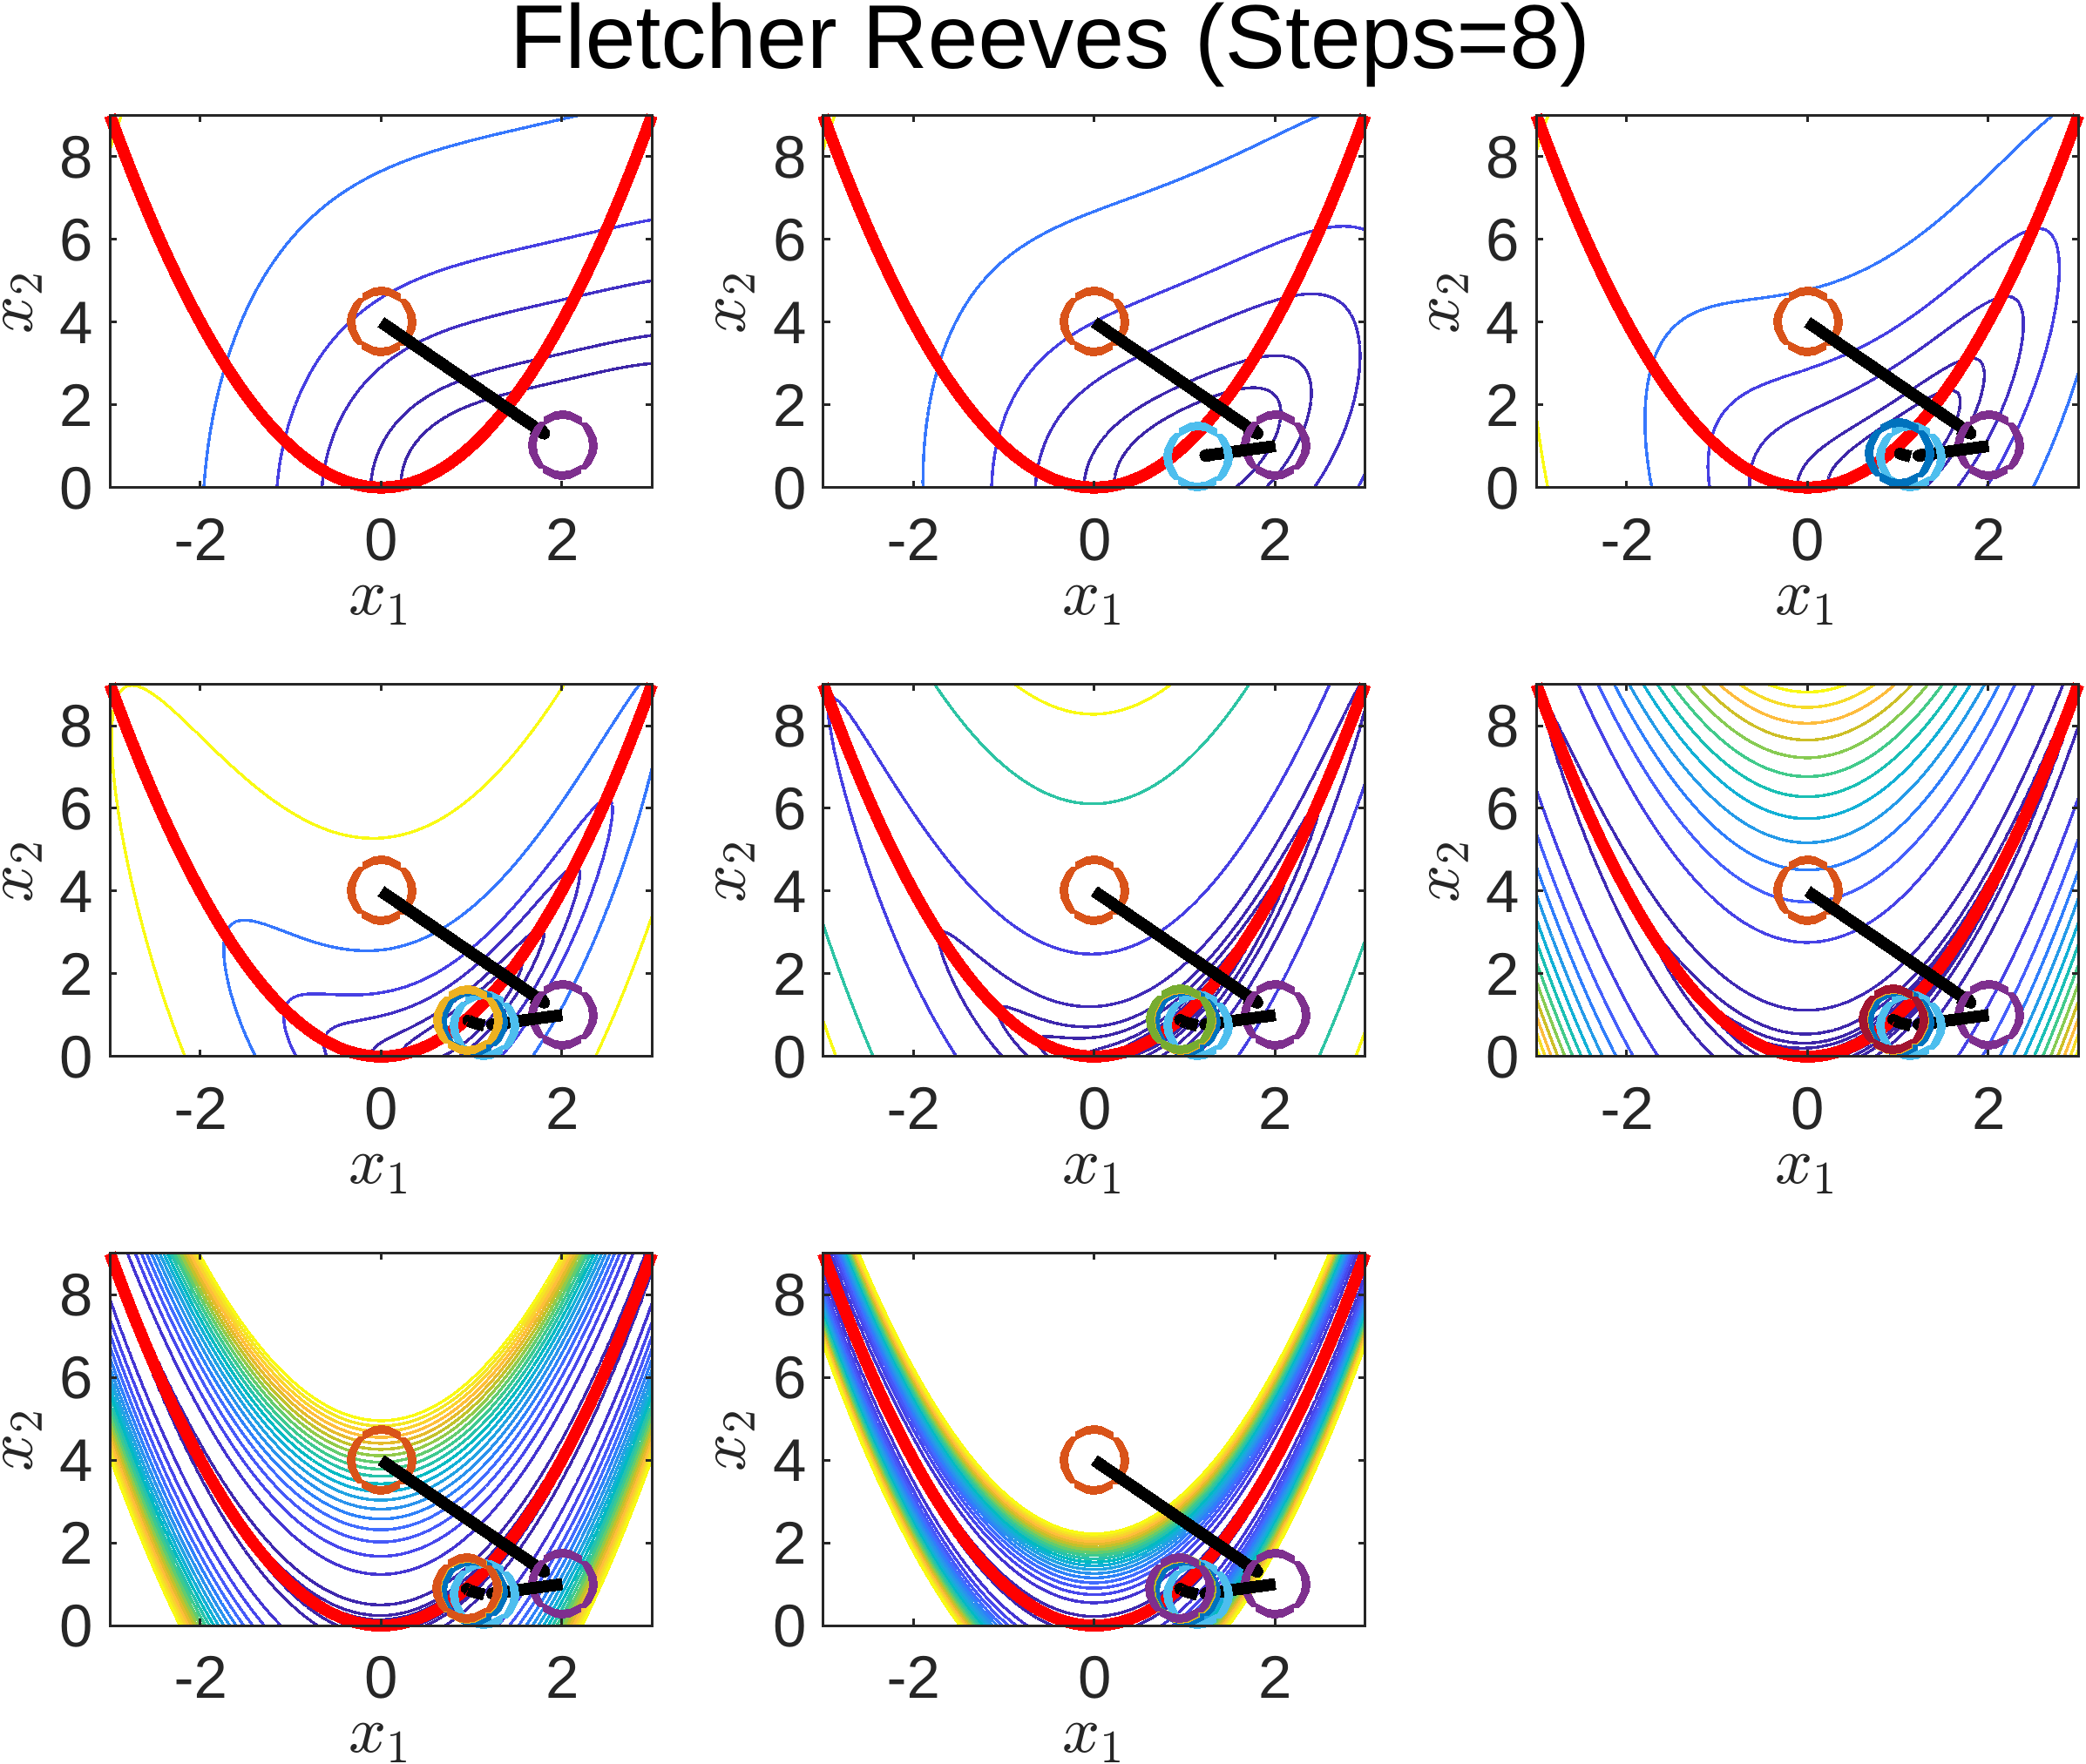
\includegraphics[width=0.65\textwidth]{fig02_P01_PEN_X2_FR.png}
      \caption{OCR do problema 01 pelo m\'etodo da penalidade, a partir do ponto $x^0=\{0,4\}$ - Algoritmo de Flecher-Reeves}
      \label{fig:fig02}
\end{figure}

Para o mesmo problema 01, a figura \ref{fig:fig03} a seguir ilustra a converg\^enia, pelo m\'etodo de OSR univariante, a partir do ponto $x^0=\{0,1\}$. Desta vez \'e poss\'ivel notar que a regi\~ao associada \`a restri\c c\~ao (curva vermelha) vai se tornando uma barreira nas curvas de n\'ivel de $\phi$. Aqui, \'e importante que a solu\c c\~ao, em qualquer passo $k$, $x^k$ permane\c ca vi\'avel, ou seja, $c_l(x^k)<=0$, caso contr\'ario, o ponto $x^k$ "romper\'a" a barreira e a fun\c c\~ao ir\'a convergir para um ponto na regi\~ao n\~ao vi\'avel.

\begin{figure}[H]
      \centering
      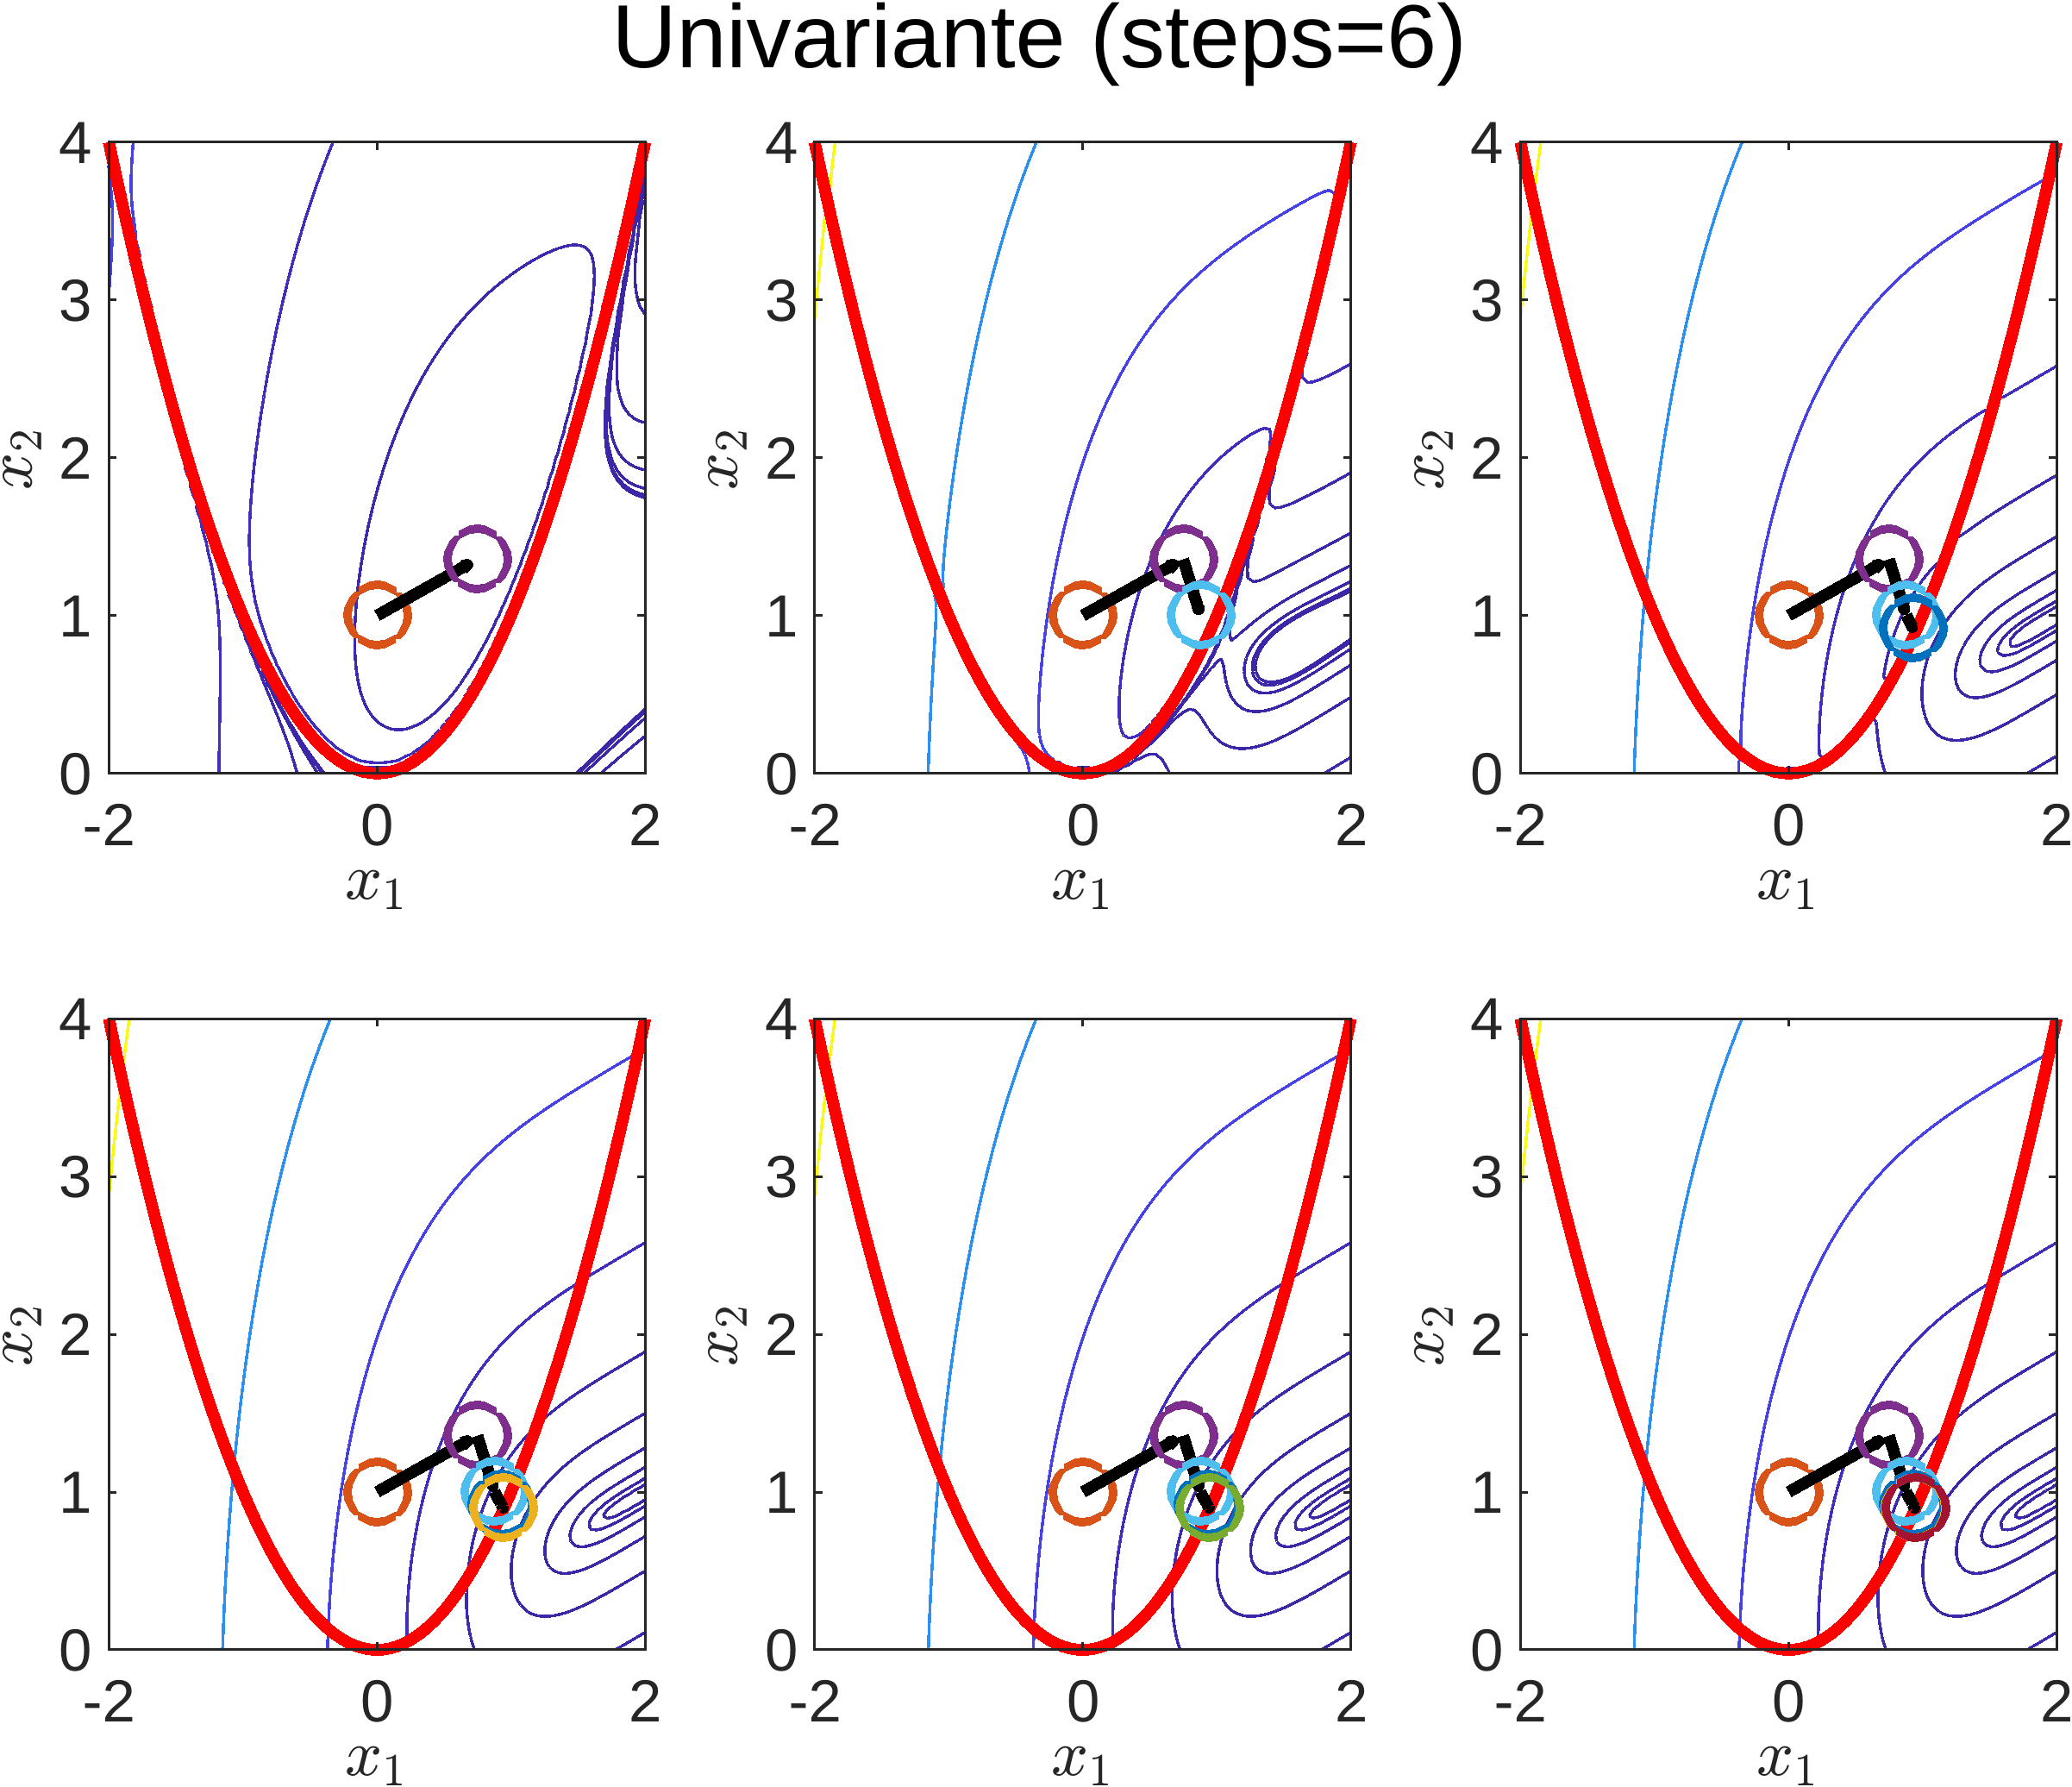
\includegraphics[width=0.65\textwidth]{fig03_P01_BAR_X1_UNI.png}
      \caption{OCR do problema 01 pelo m\'etodo da barreira, a partir do ponto $x^0=\{0,1\}$ - Algoritmo Univariante}
      \label{fig:fig03}
\end{figure}

\newpage
Para melhor visualiza\c c\~ao da pseudo-fun\c c\~ao objetivo acima plotamos os gr\'aficos de curvas de n\'ivel e 3D da fun\c c\~ao da eq. \ref{eqPhi1B} nas figuras \ref{fig:wolf_contour} e \ref{fig:wolf_3d}, respectivamente, onde fica claro a regi\~ao associada \`a restri\c c\~ao como sendo uma "descontinuidade" de $\phi$ e porque o m\'etodo \'e chamado de m\'etodo de barreira.

\begin{equation} \label{eqPhi1B}
      \phi (x,y, r_b=1) = (x-2)^4 + (x-2y)^2 - \frac{rb}{x^2-y}
\end{equation}

\begin{figure}[H]
      \centering
      \begin{subfigure}{0.35\textwidth}
            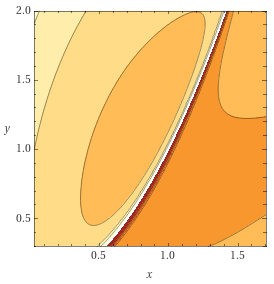
\includegraphics[width=\textwidth]{wolf_contour.PNG}
            \caption{contono de $\phi$}
            \label{fig:wolf_contour}
      \end{subfigure}
      \begin{subfigure}{0.45\textwidth}
            \centering
            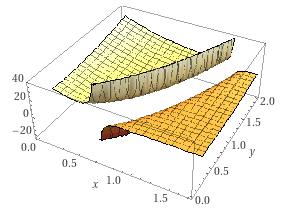
\includegraphics[width=\textwidth]{wolf_3d.PNG}
            \caption{3D plot de $\phi$}
            \label{fig:wolf_3d}
      \end{subfigure}
      \caption{Pseudo fun\c c\~ao objetivo do problema 01 (Barreira) com $rb=1$ (equa\c c\~ao \ref{eqPhi1B}), https://www.wolframalpha.com}
      \label{fig:wolf}
\end{figure}

Para avaliar a robustez do m\'etodo, selecionamos um novo ponto $x^0=\{2.5,10\}$, ainda vi\'avel, Na figura \ref{fig:fig04} ilustra-se tal caso pelo m\'etodo de Steepest-Descent.

\begin{figure}[H]
      \centering
      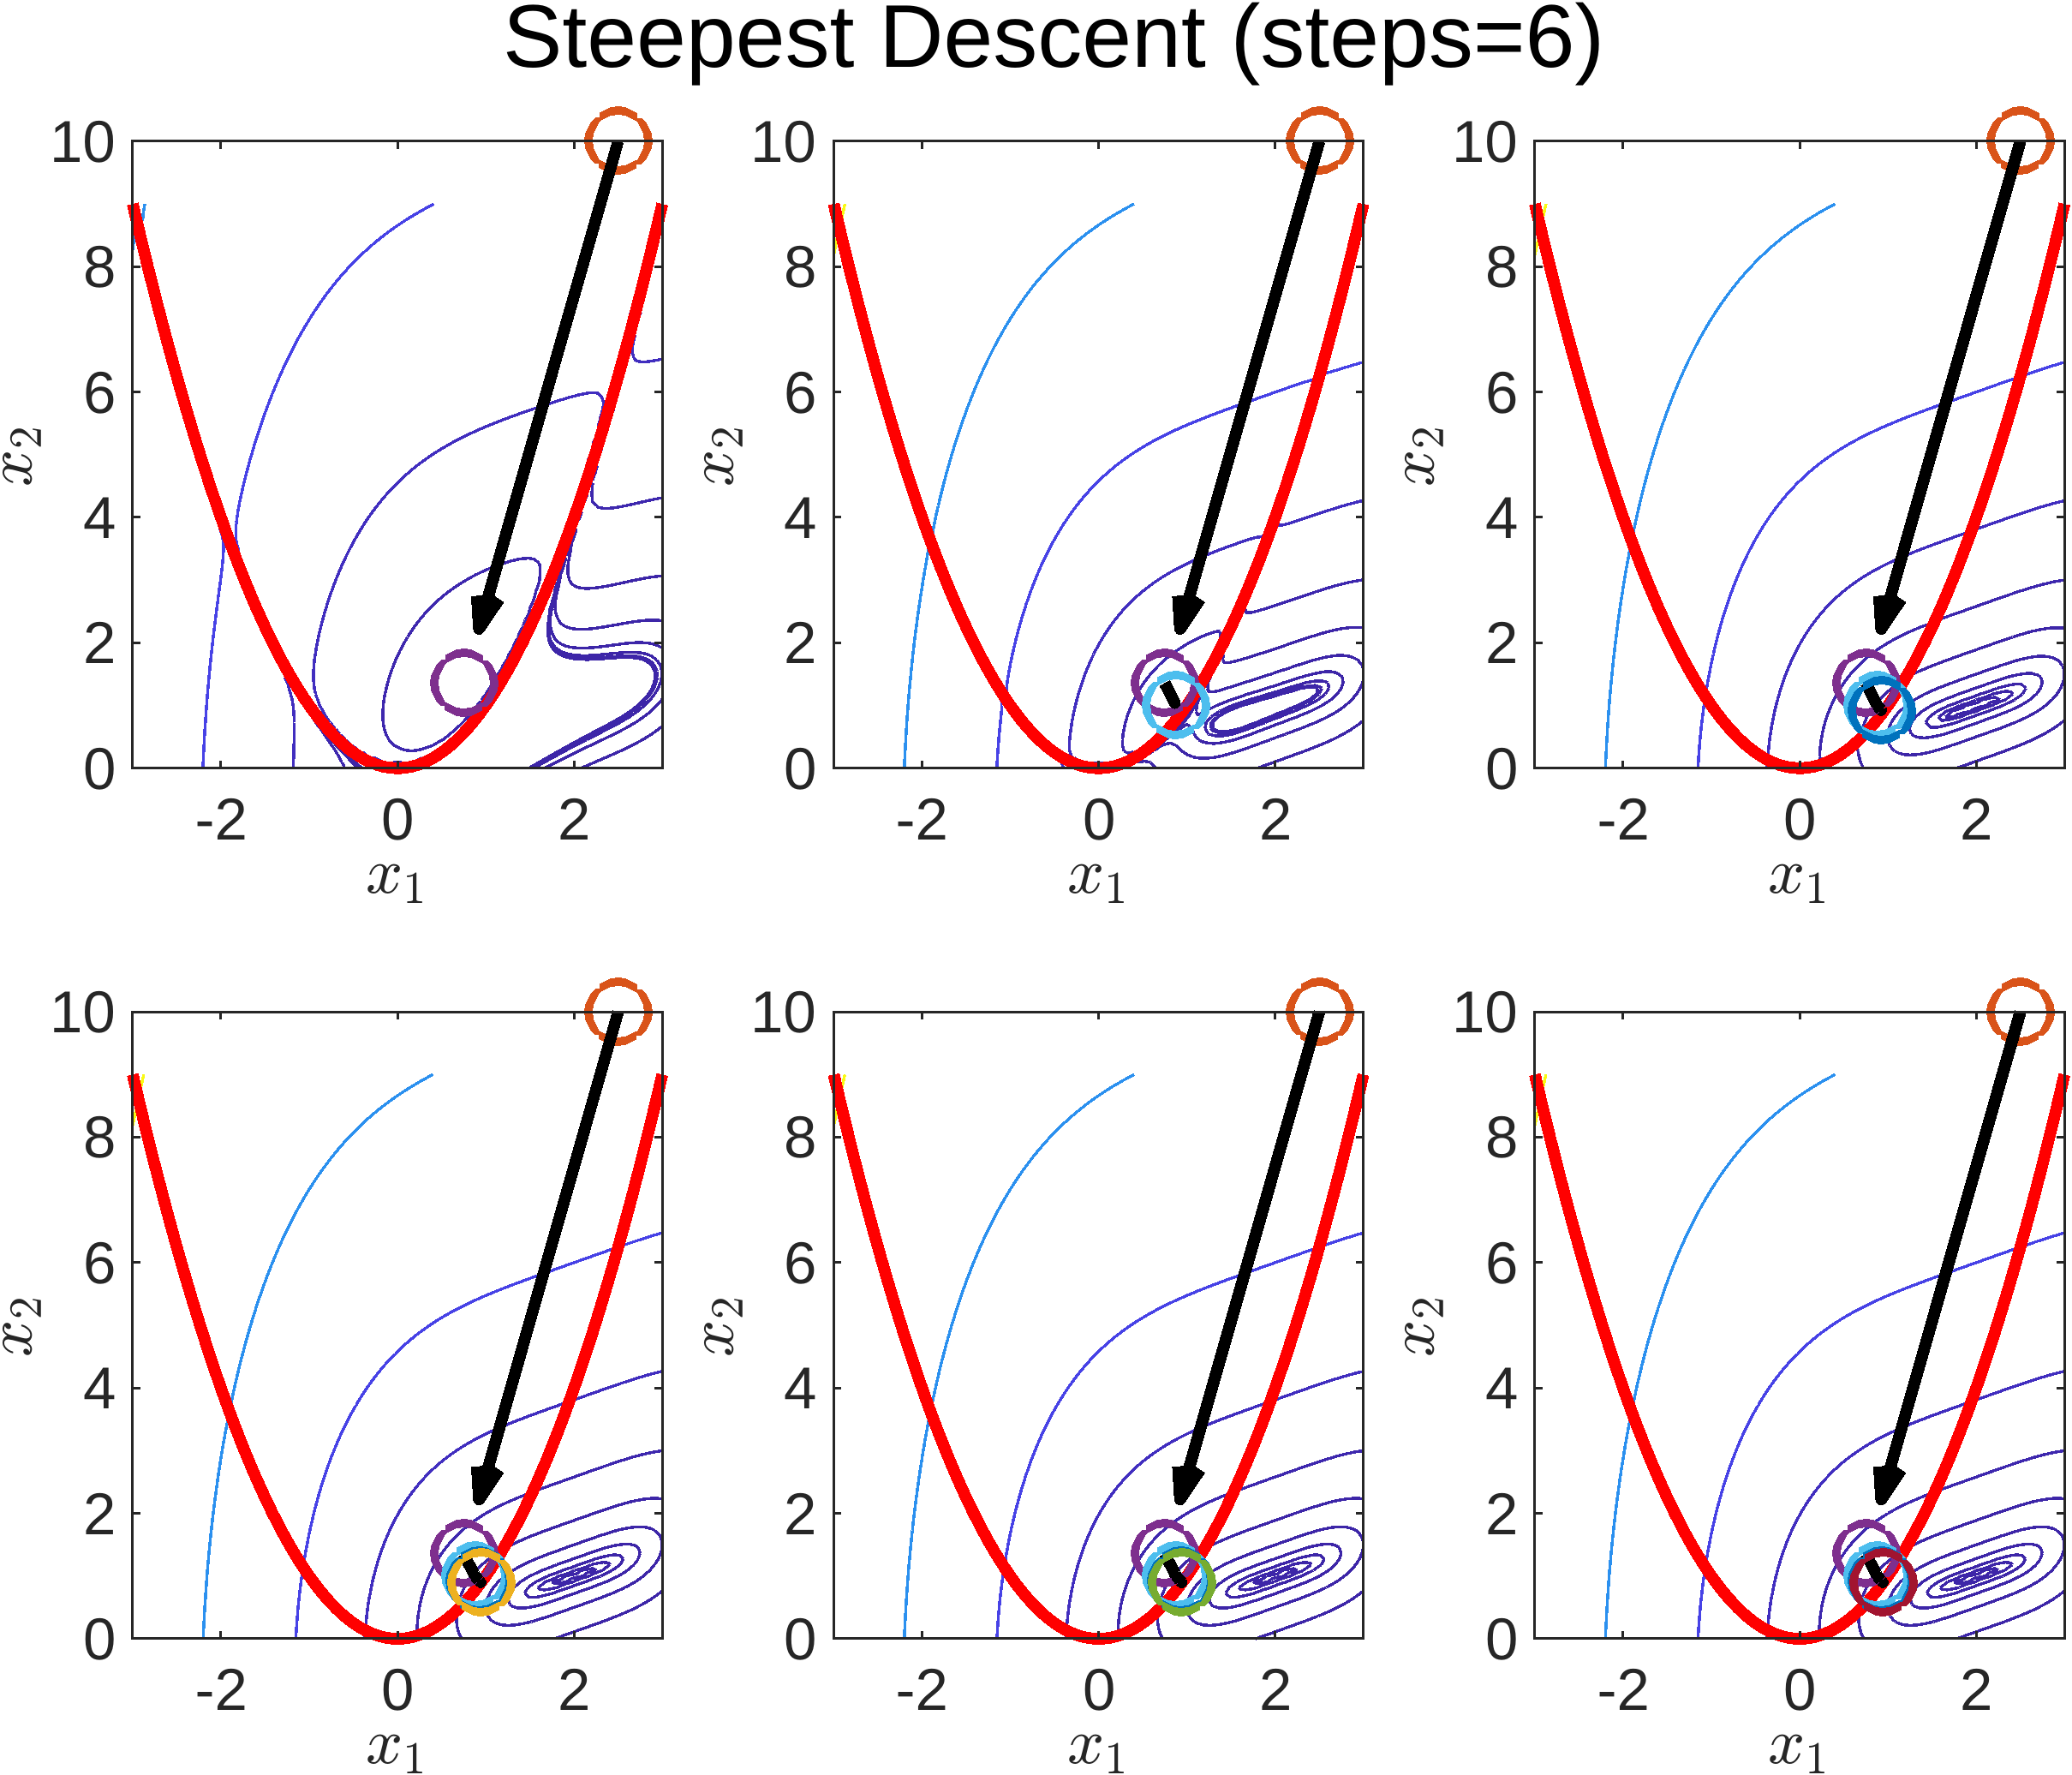
\includegraphics[width=0.65\textwidth]{fig04_P01_BAR_X2_SD.png}
      \caption{OCR do problema 01 pelo m\'etodo da barreira, a partir do ponto $x^0=\{2.5,10\}$ - Algoritmo Steepest Descent}
      \label{fig:fig04}
\end{figure}

\newpage
%%%%%%%%%%%%%%%%%%%%%%%%%%%
% PROBLEMA 02
%%%%%%%%%%%%%%%%%%%%%%%%%%%

As figuras a seguir ilustram as curvas da solu\c c\~ao de OCR para a fun\c c\~ao a as restri\c c\~oes do problema 2

Nas figuras \ref{fig:fig05} e \ref{fig:fig06} a seguir ilustra-se as converg\^encias do algoritmo de OCR pelo m\'etodo de penalidade para dois pontos de partida distintos: $x^0=\{1,15\}$ e $x^0=\{3,3\}$, respecivamente. O primeiro utilizando, para OSR o m\'etodo de dire\c c\~oes de busca de Fletcher-Reeves e o segundo, Univariante.

Nota-se nesses dois gr\'aficos a maior complexidade da fun\c c\~ao e o consequente maior n\'umero de passos necess\'arios para converg\^encia.

\begin{figure}[H]
      \centering
      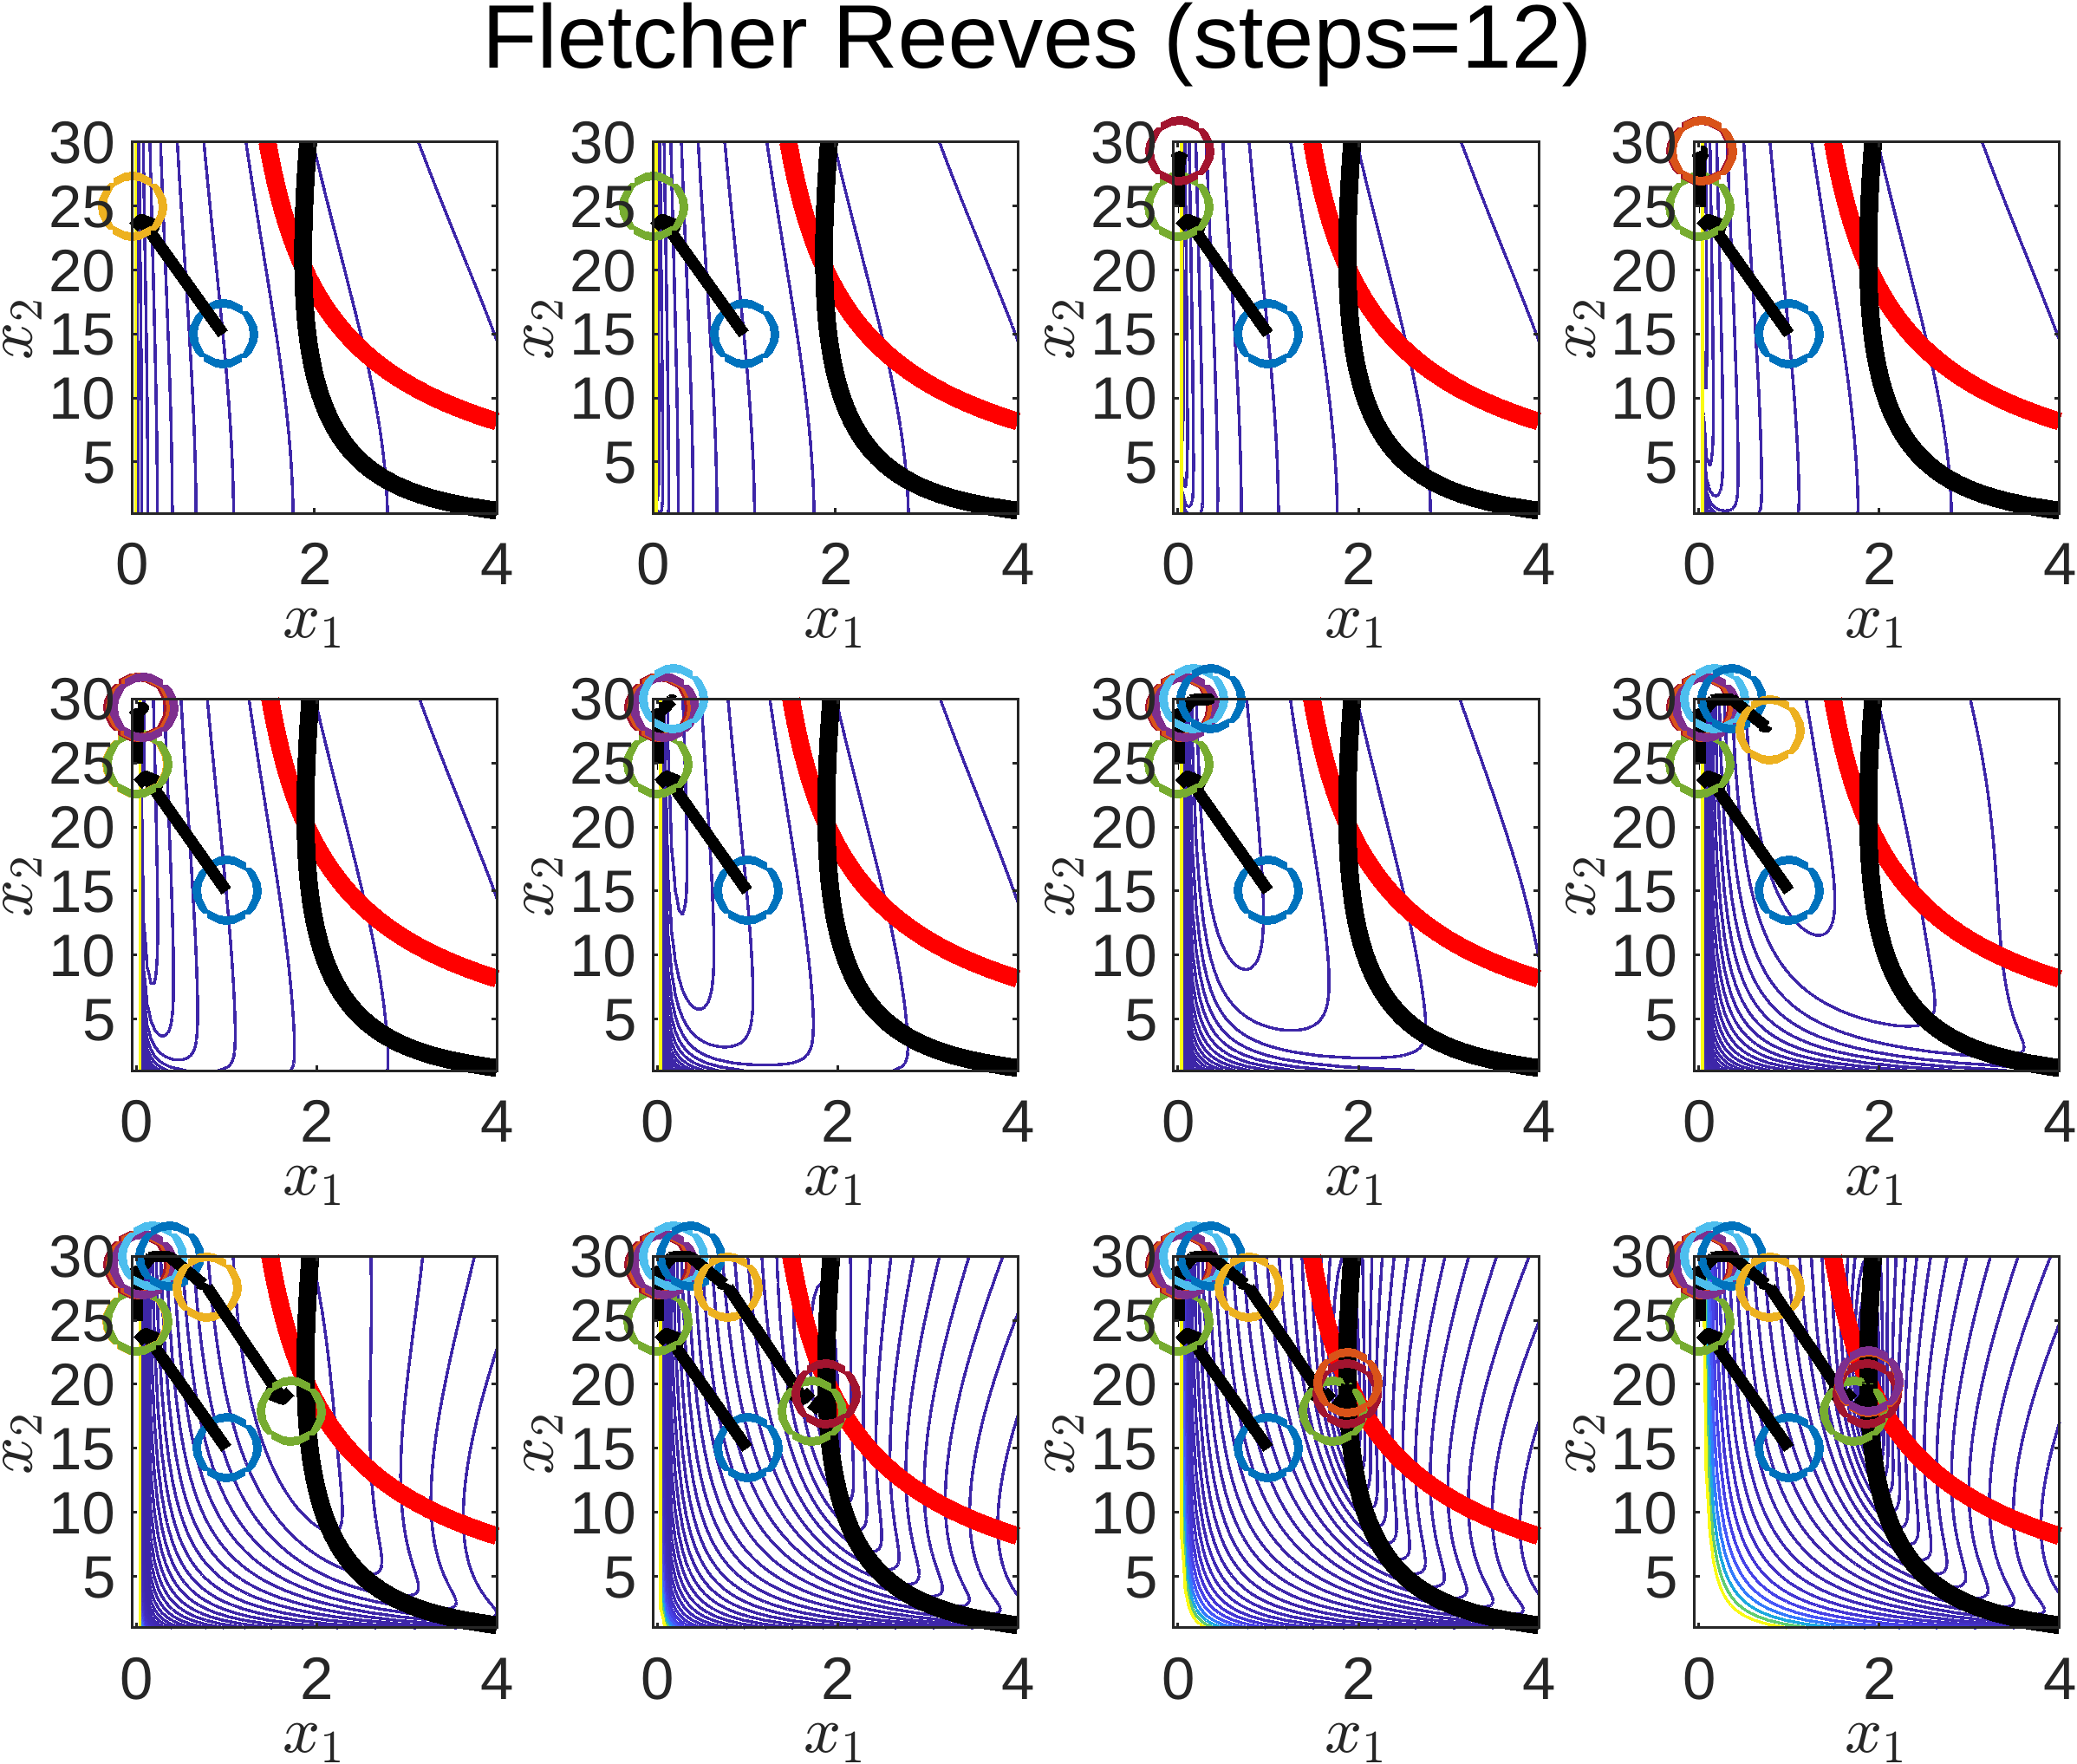
\includegraphics[width=0.65\textwidth]{fig05_P02_PEN_X1_FR.png}
      \caption{OCR do problema 02 pelo m\'etodo da penalidade, a partir do ponto $x^0=\{1,15\}$ - Algoritmo de Flecher-Reeves}
      \label{fig:fig05}
\end{figure}
\begin{figure}[H]
      \centering
      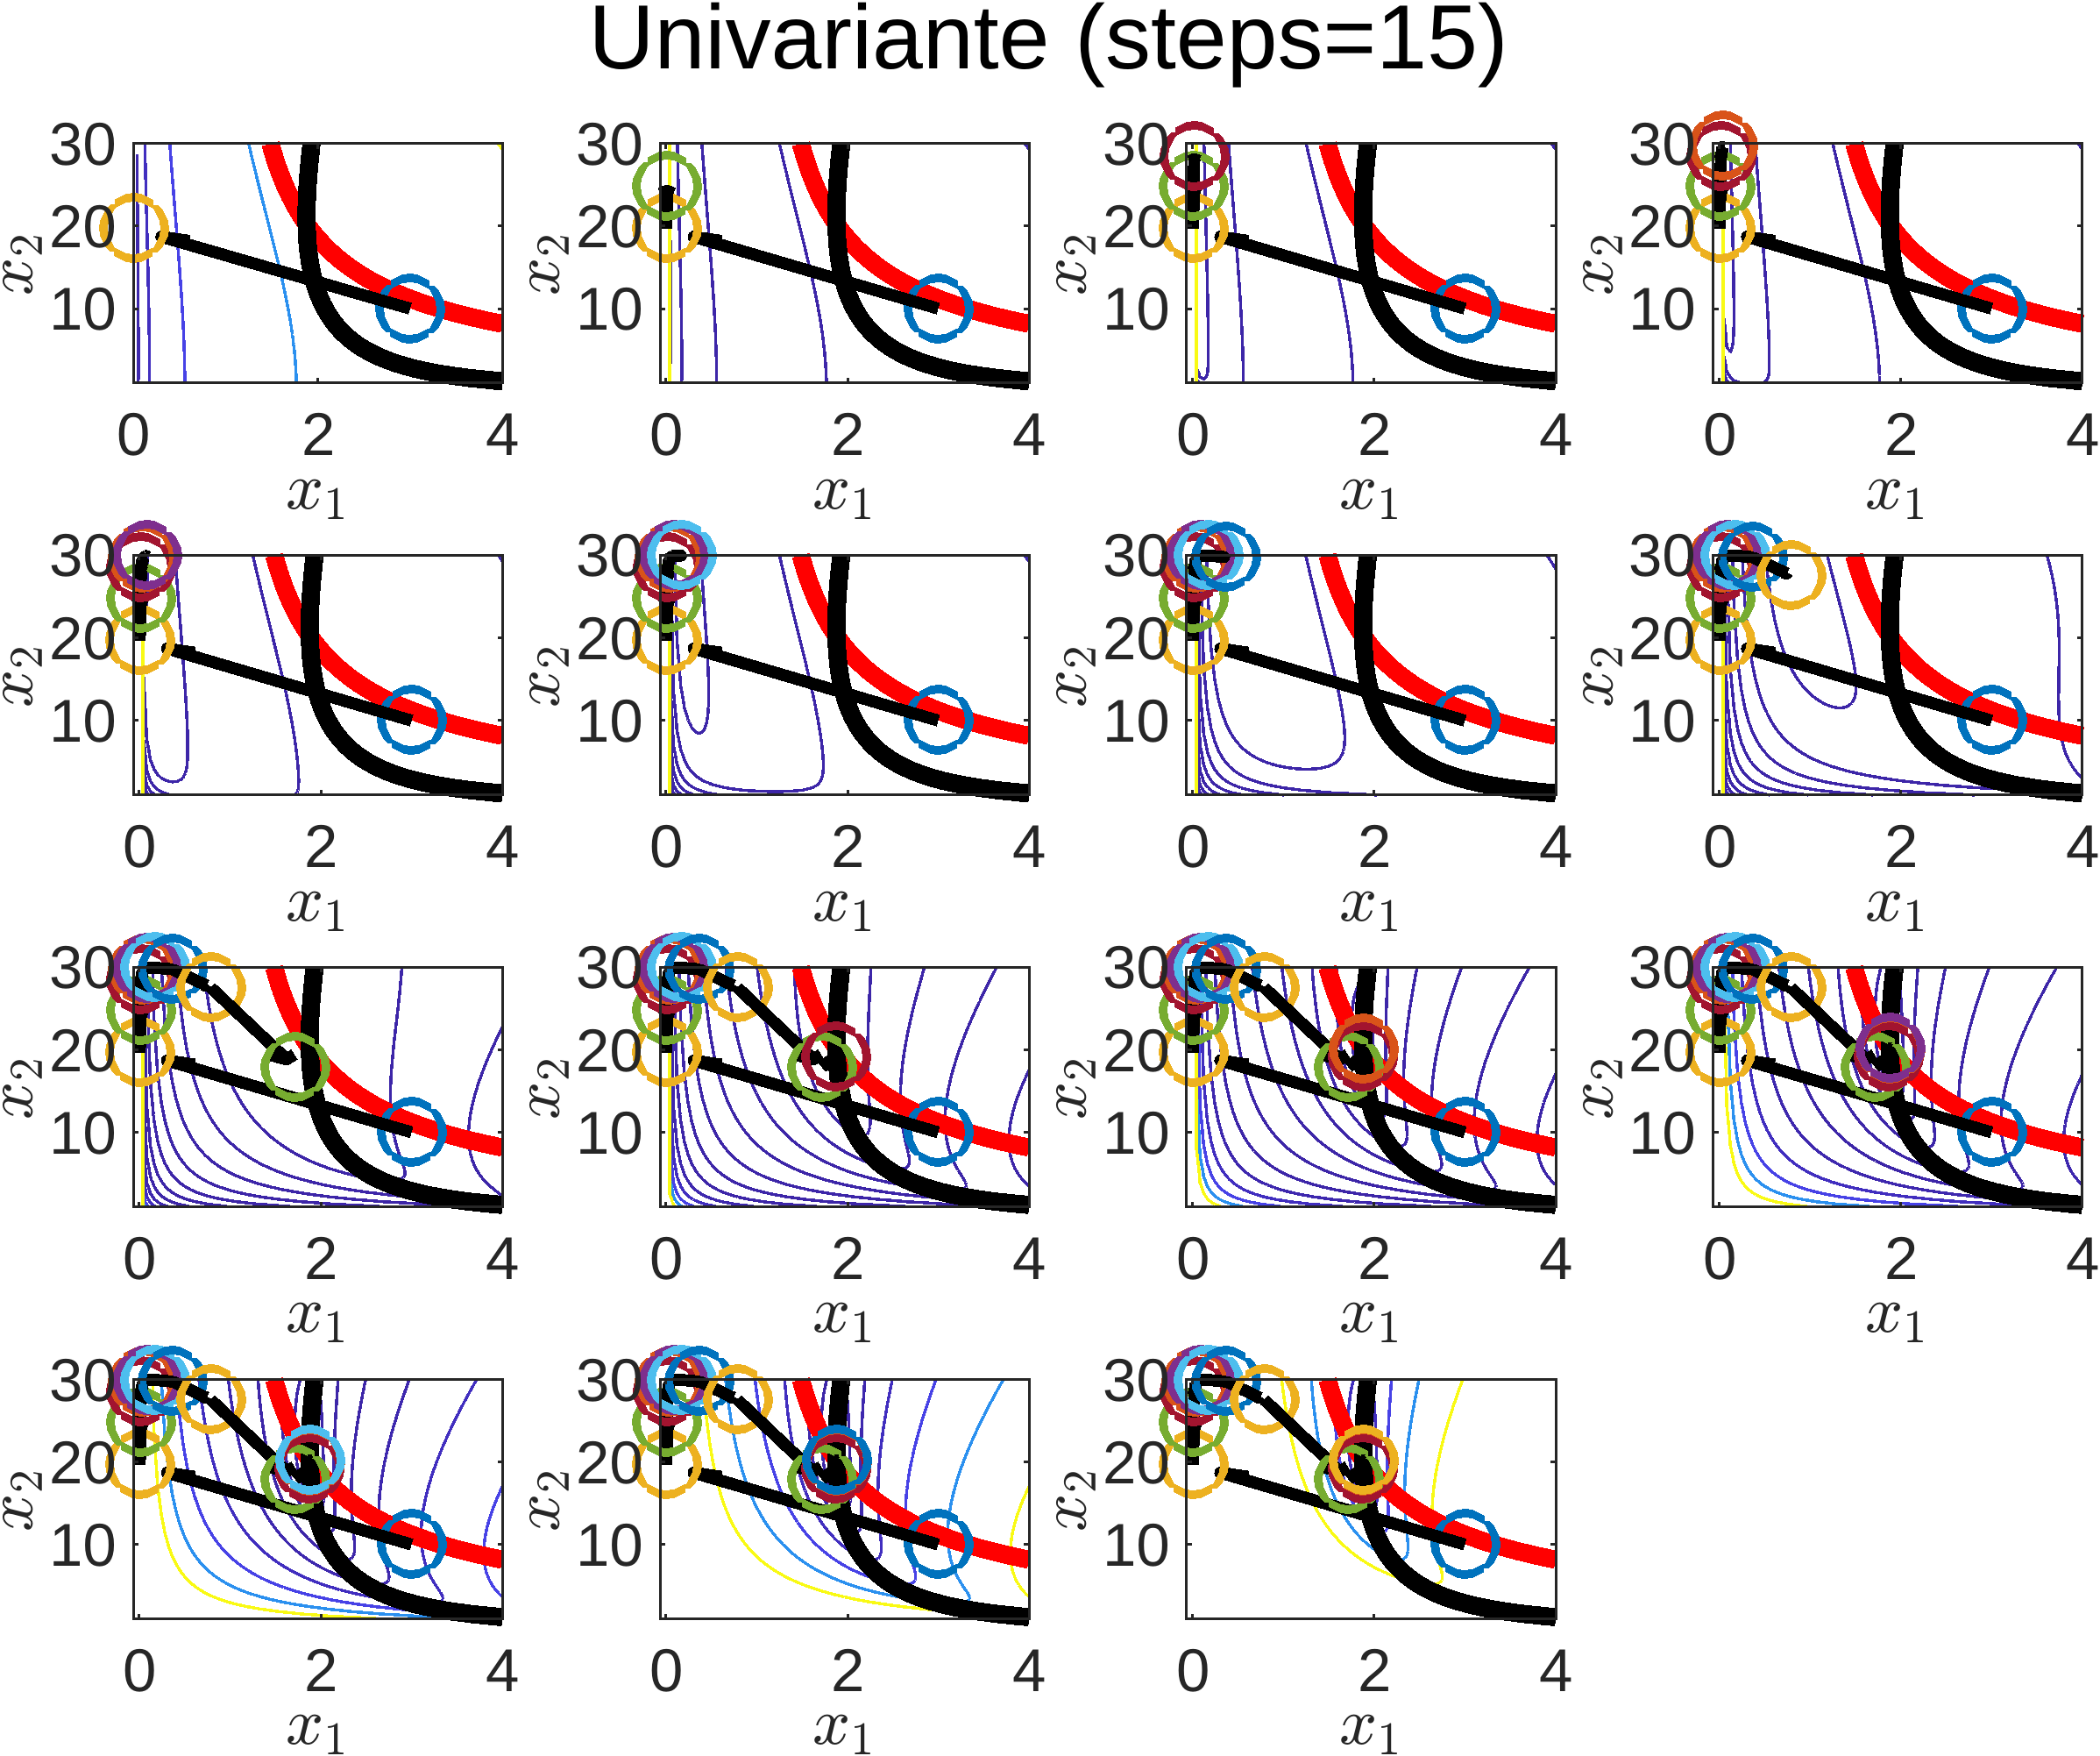
\includegraphics[width=0.65\textwidth]{fig06_P02_PEN_X2_UNI.png}
      \caption{OCR do problema 02 pelo m\'etodo da penalidade, a partir do ponto $x^0=\{3,3\}$ - Algoritmo Univariante}
      \label{fig:fig06}
\end{figure}

\newpage

Nas figuras \ref{fig:fig07} e \ref{fig:fig08} a seguir ilustra-se as converg\^encias do algoritmo de OCR pelo m\'etodo de barreira para dois pontos de partida distintos: $x^0=\{4,25\}$ e $x^0=\{10,5\}$, respecivamente. O primeiro utilizando, para OSR o m\'etodo de dire\c c\~oes de busca de Newton-Raphson e o segundo, Fletcher-Reeves.

\begin{figure}[H]
      \centering
      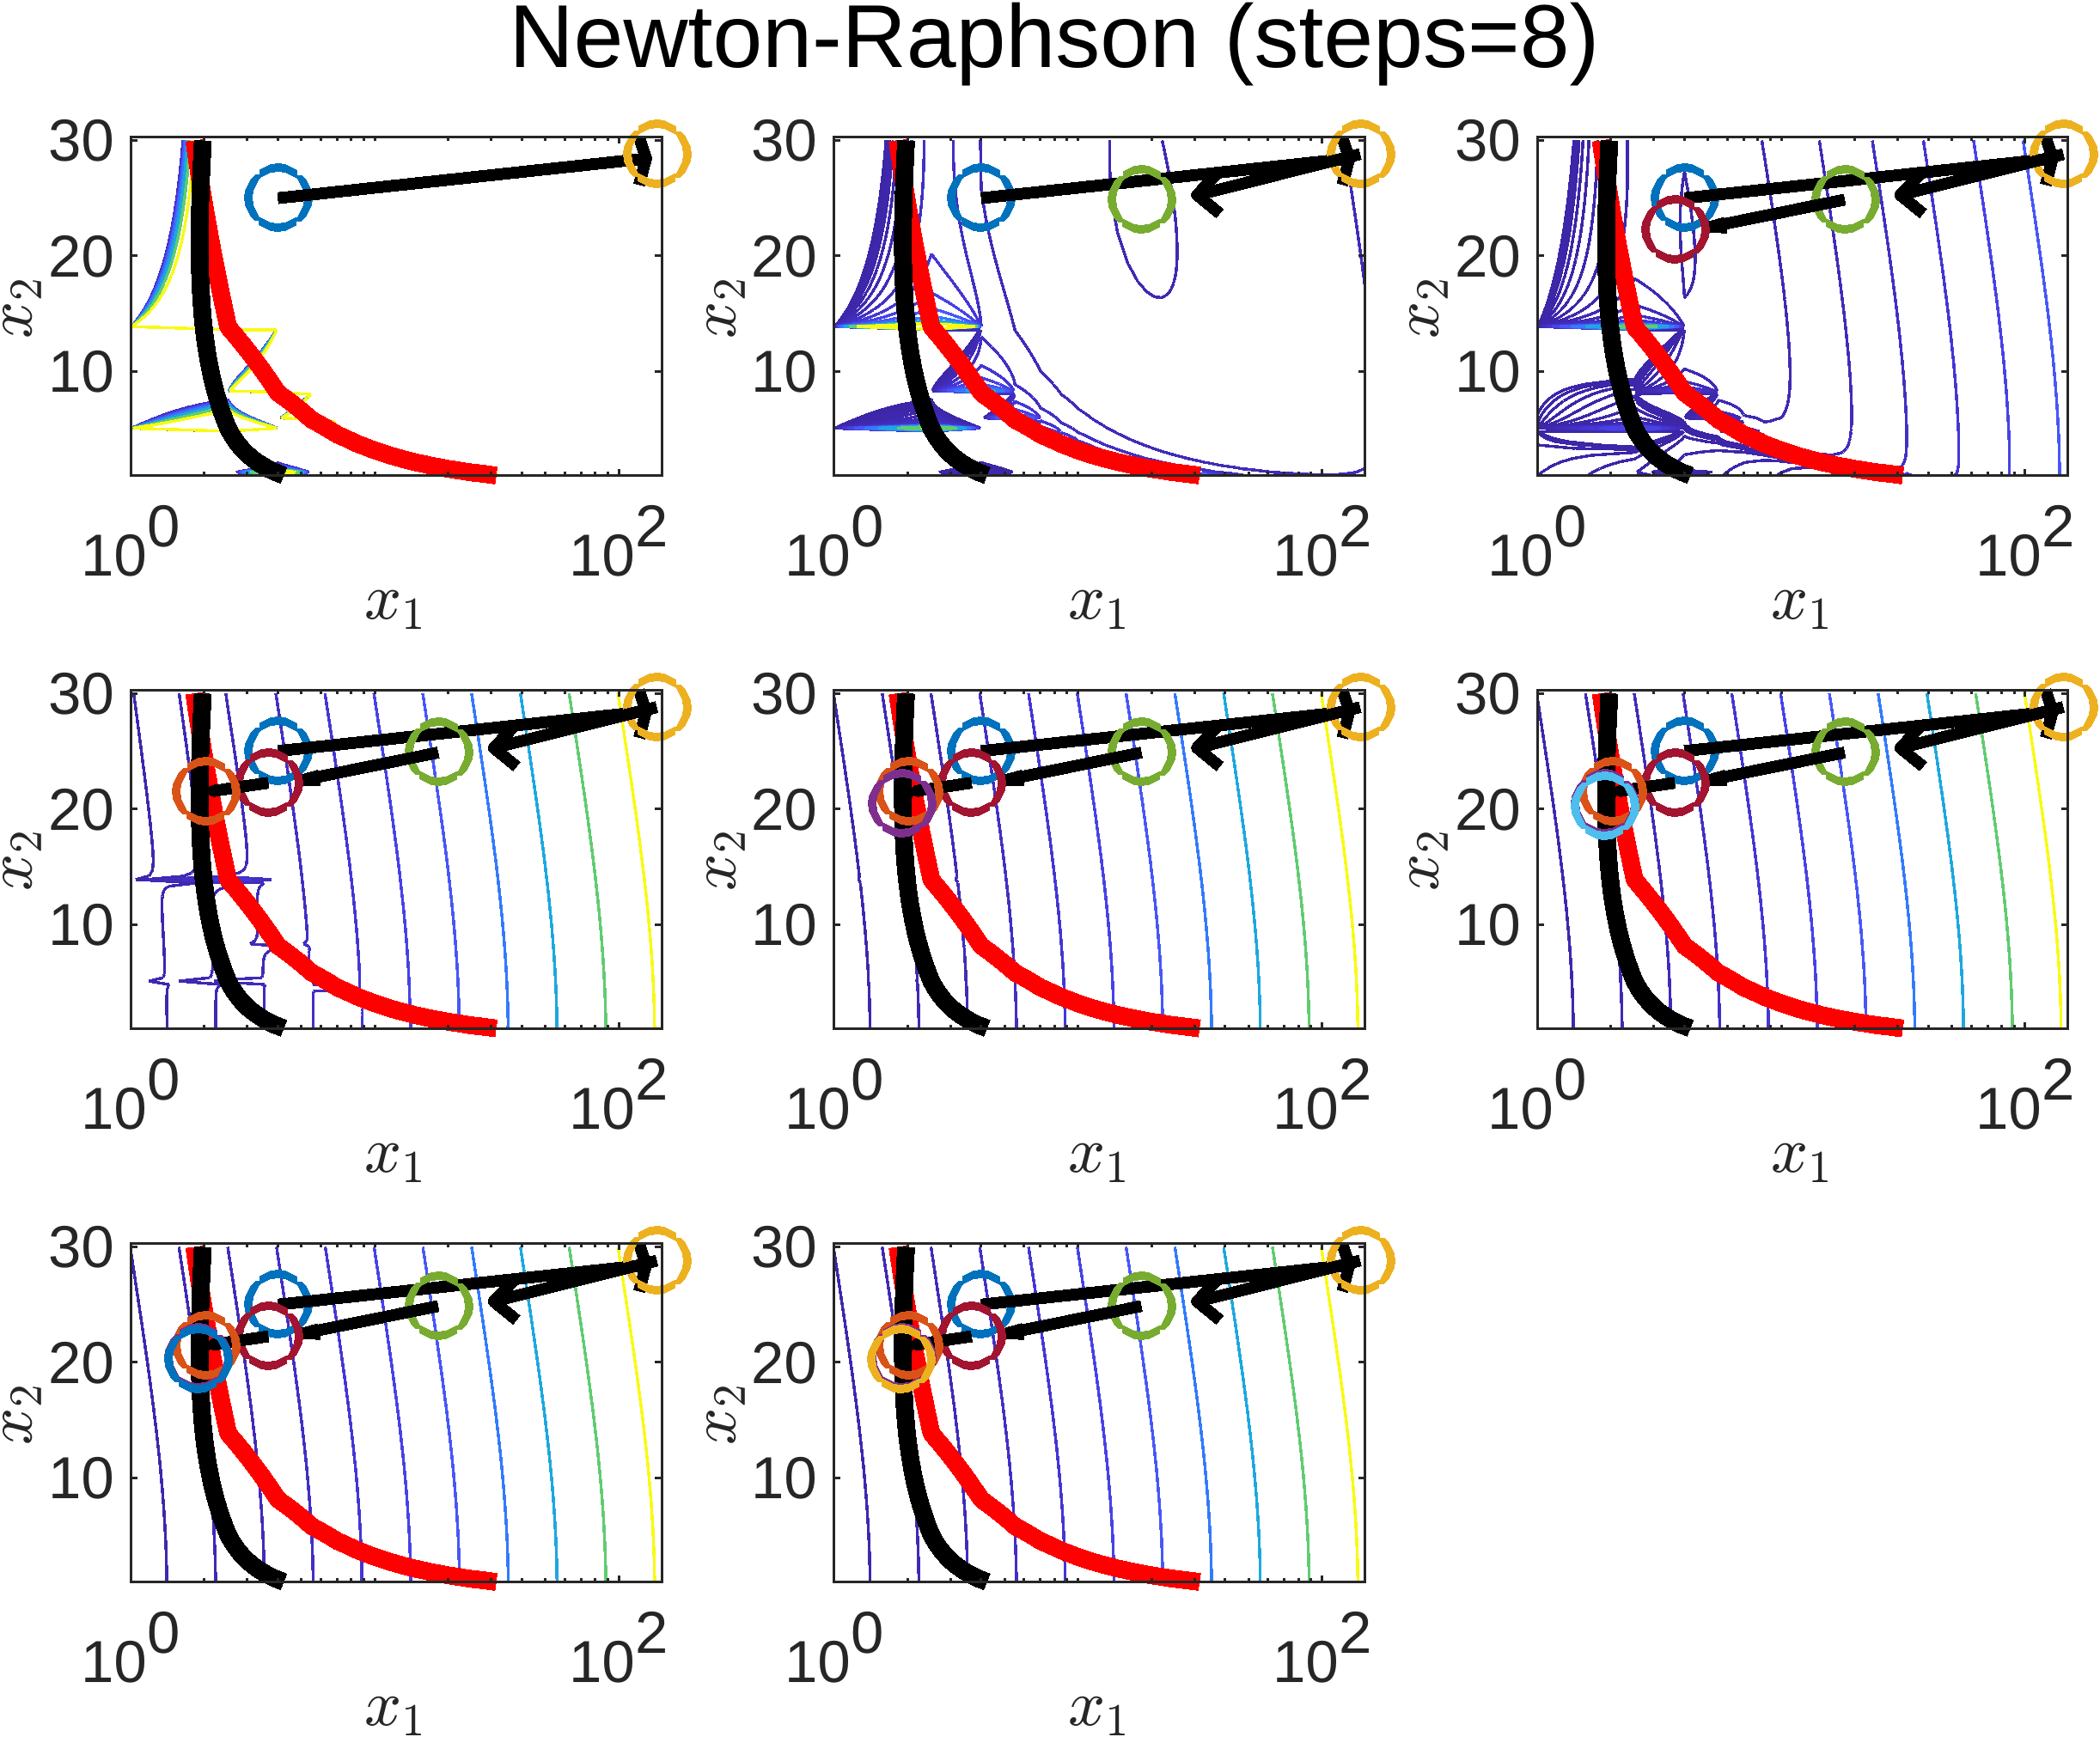
\includegraphics[width=0.65\textwidth]{fig07_P02_BAR_X1_NR.png}
      \caption{OCR do problema 02 pelo m\'etodo da barreira, a partir do ponto $x^0=\{4,25\}$ - Algoritmo de Newton-Raphson}
      \label{fig:fig07}
\end{figure}
\begin{figure}[H]
      \centering
      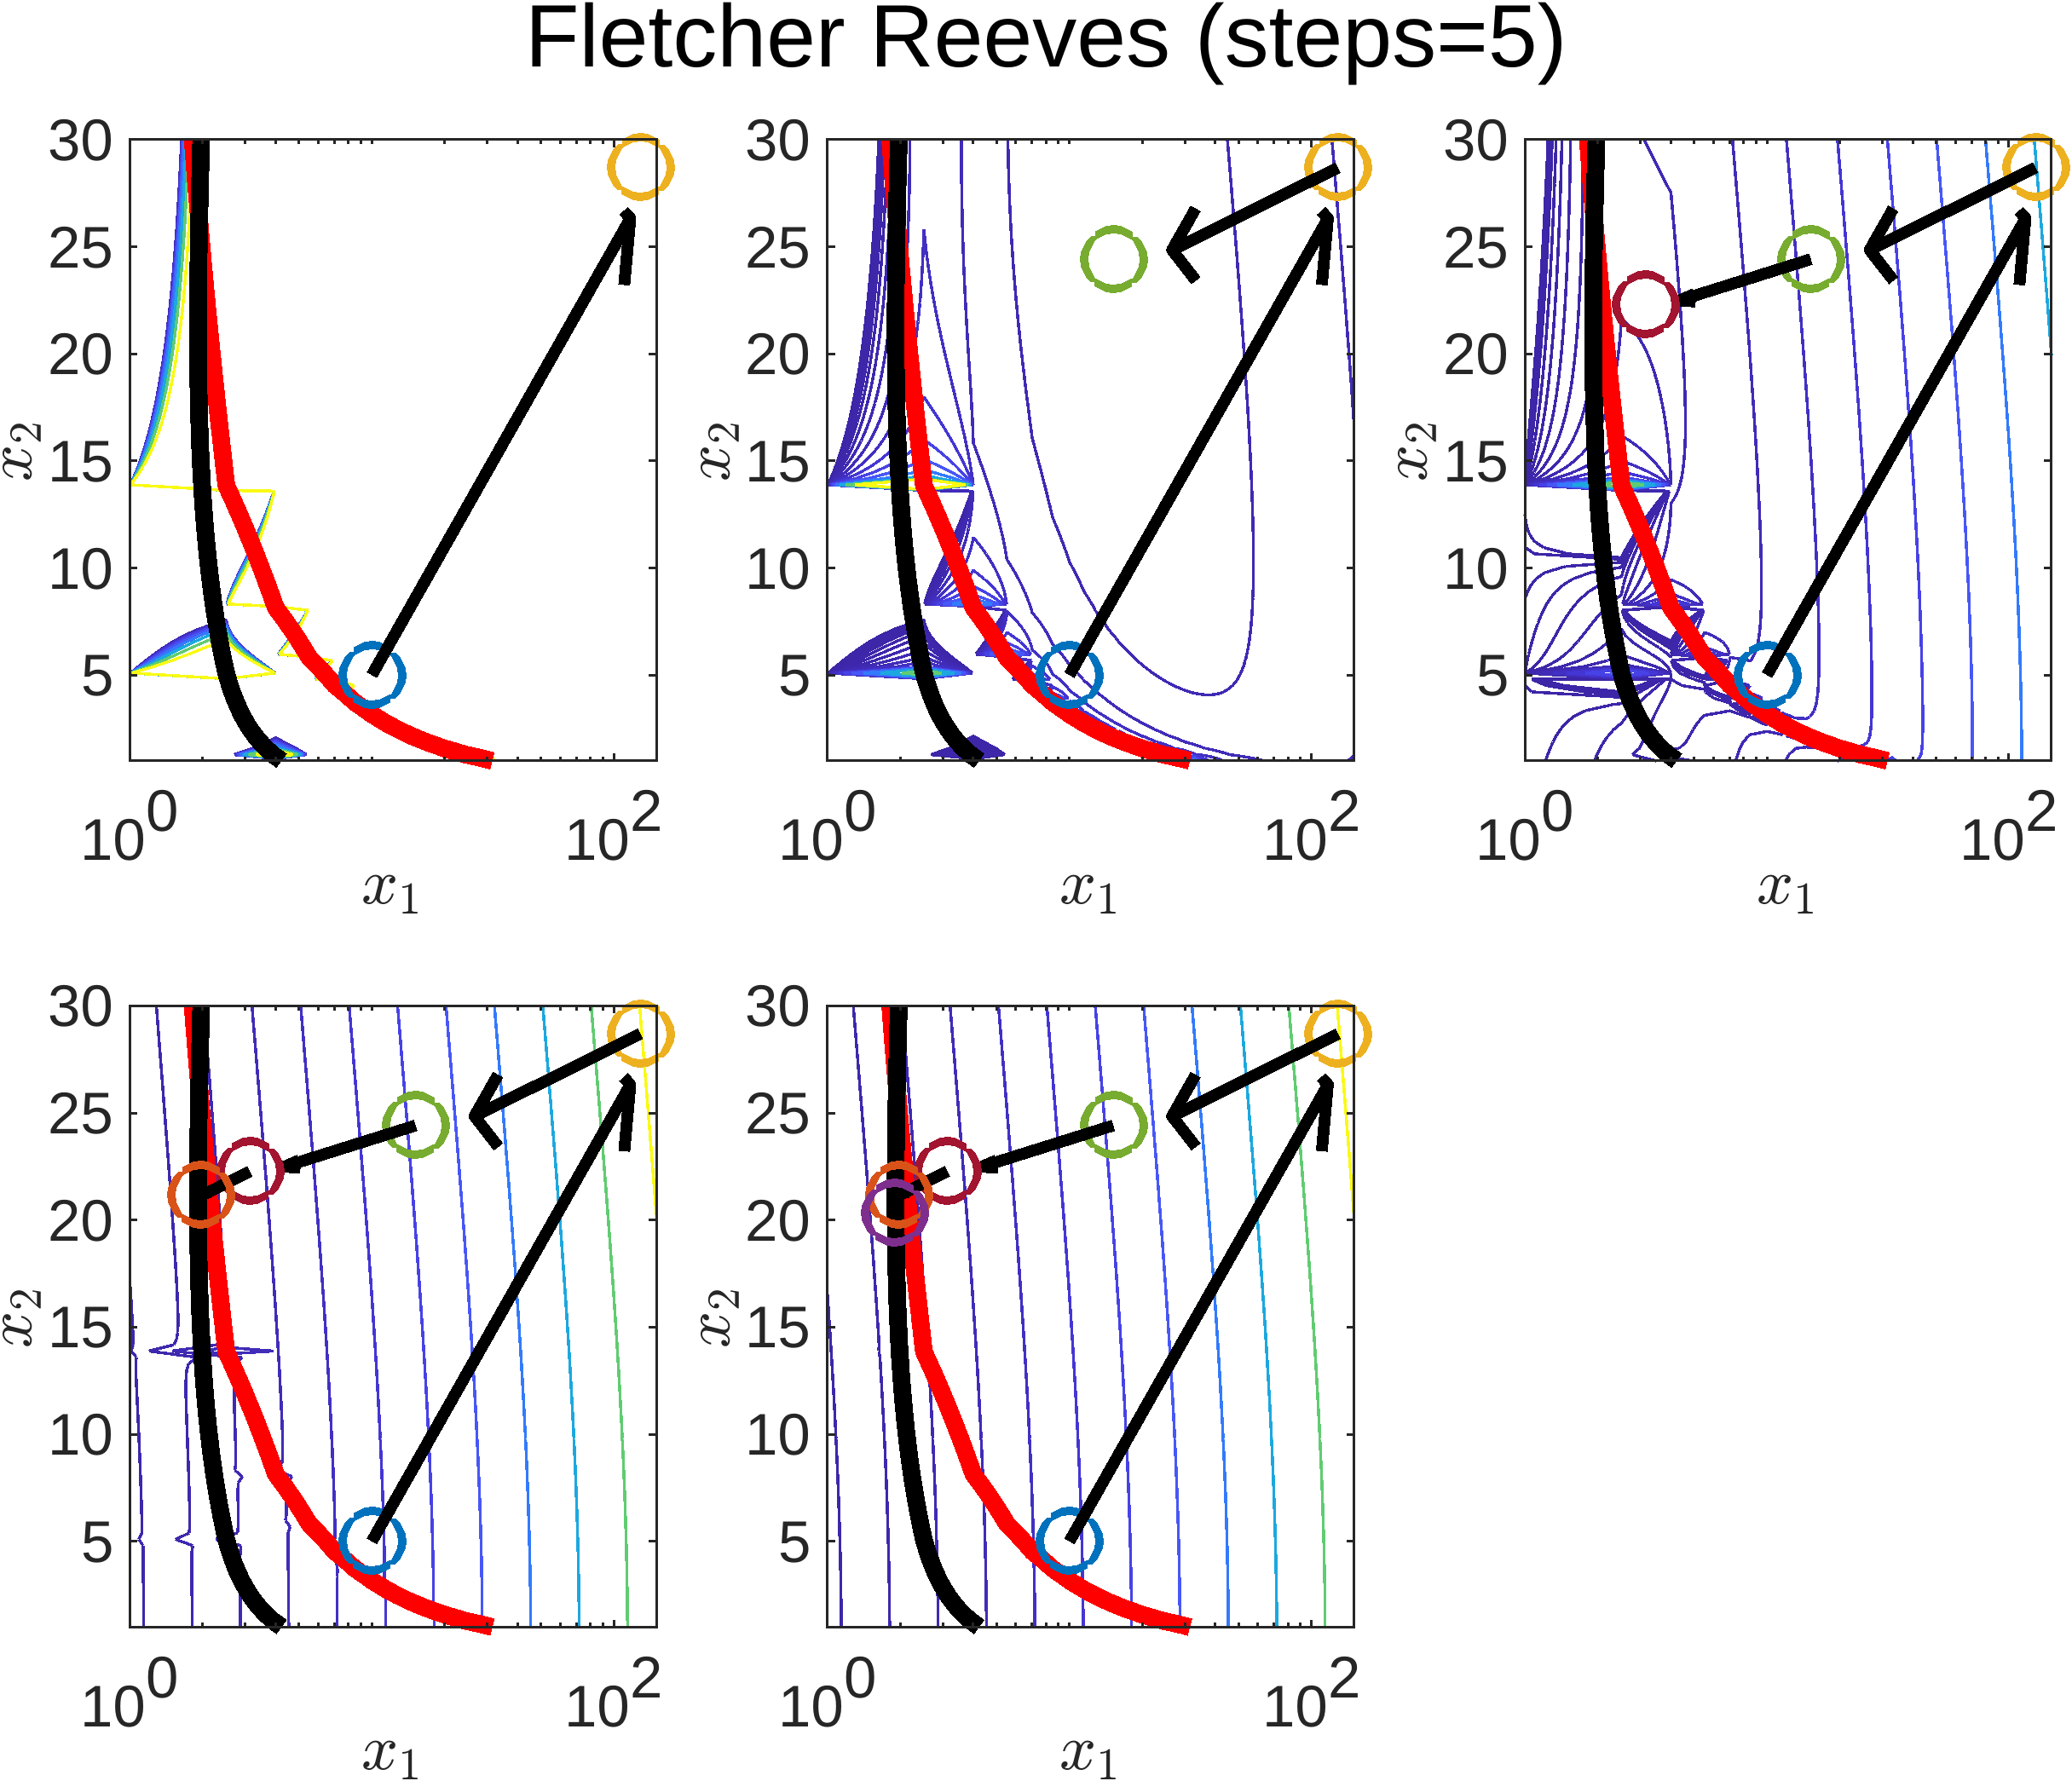
\includegraphics[width=0.65\textwidth]{fig08_P02_BAR_X2_FR.png}
      \caption{OCR do problema 02 pelo m\'etodo da barreira, a partir do ponto $x^0=\{10,5\}$ - Algoritmo de Fletcher-Reeves}
      \label{fig:fig08}
\end{figure}


\section{Conclus\~oes}

A realiza\c c\~ao deste trabalho permitiu implementar os m\'etodos estudados na disciplina de otimiza\c c\~ao. Para todos os casos de aplica\c c\~ao, foram rodados os algortimos para outros pontos que n\~ao os pontos propostos no problema em si e cujo resultado mostrou que os algortimos de busca e miniza\c c\~ao s\~ao robustos, mesmo nos casos de fun\c c\~oes n\~ao quadr\'aticas.

Em alguns poucos casos o algoritmo n\~ao obteve o resultado esperado em rela\c c\~ao ao n\'umero de passos at\'e a converg\^encia. Em geral, notou-se que a converg\^encia, n\'umero de passos e o tempo de execu\c c\~ao dos algoritmos \'e muito sens\'ivel a escolha de seus par\^metros, o que reside nas incertezas num\'ericas associadas aos m\'etodos de busca linear, principalmente.

Em um dos m\'etodos (Newton-Raphson) foi encontrado um ponto de cela e n\~ao um ponto de m\'inimo, mas este \'e um comportamento esperado do algoritmo j\'a que o mesmo se prop\~oe apenas a identificar os pontos cr\'iticos, candidatos a m\'inimo de $f$, sem entrar na avalia\c c\~ao da hessiana.

\section{Anexos}

A seguir est\~ao ilustrados alguns dos c\'odigos ou trechos de c\'odigos decritos na se\c c\~ao metodologia.

\begin{minipage}{\linewidth}
      \begin{lstlisting}[style=myStyle, caption=script t01.m setando par\^ametros e criando as fun\c c\~oes, label=l1]
            % dados do item 01a, f, grad f, hess f e x0
            fa = @(x) x(1)^2-3*x(1)*x(2)+4*x(2)^2+x(1)-x(2);
            gfa = @(x) [2*x(1)-3*x(2)+1 ; -3*x(1)+8*x(2)-1];
            Ha = @(x) [2 -3;-3 8];
            x01 = [2;2];
            x02 = [-1;-3];
            % parametros dos algoritmos
            iter_max = 100;
            a = 0.002; % passo
            TOL = 1e-4; % parada do gradiente
            TOL2 = 1e-7; % busca linear
            methods = ["Univariante","Powell","Steepest Descent","Fletcher Reeves","Newton-Raphson","BFGS"];
      \end{lstlisting}
\end{minipage}

\begin{minipage}{\linewidth}
      \begin{lstlisting}[style=myStyle, caption=script t01.m chamando o script osr.m para a fun\c c\~ao do item 1a para cada um dos 6 m\'etodos estudados, label=l2]
            fprintf('\n******************** ITEM 01A ************************\n');
            for method = 1:6
                fprintf('---%s---\n', methods(method));

                fprintf('x0=[%2d,%2d]: ',x01(1), x01(2));
                [x_1,t] = osr (fa, gfa, Ha, x01, method, iter_max, a, TOL, TOL2);
                fprintf('(%.1fms), xmin=[%0.4f,%0.4f], f=%0.4f\n', t*1000, x_1(1,end), x_1(2,end), fa(x_1(:,end)));

                fprintf('x0=[%2d,%2d]: ',x02(1), x02(2));
                [x_2,t] = osr (fa, gfa, Ha, x02, method, iter_max, a, TOL, TOL2);
                fprintf('(%.1fms), xmin=[%0.4f,%0.4f], f=%0.4f\n', t*1000, x_2(1,end), x_2(2,end), fa(x_2(:,end)));

                plot_result(min([x_1(1,:), x_2(1,:)])-dx,max([x_1(1,:), x_2(1,:)])+dx,min([x_1(2,:), x_2(2,:)])-dx,max([x_1(2,:), x_2(2,:)])+dx, x_1, x_2, methods(method), 1)
                exportgraphics(gcf,strcat('./figures/img01A_m0',num2str(method),'.png'),'Resolution',500)
            end
      \end{lstlisting}
\end{minipage}

\begin{minipage}{\linewidth}
      \begin{lstlisting}[style=myStyle, caption=script osr.m implementando o m\'etodo de Powell, label=list_osr]
            function [x_,time_elap] = osr (f, gf, H, x0, method, iter_max, a, TOL, TOL2)
            % 1. Univariante
            % 2. Powell
            % 3. Steepest Descent
            % 4. Flecher?Reeves
            % 5. Newton?Raphson
            % 6. BFGS

            k=0;
            conv=0; %flag convergencia
            tstart = tic;
            switch method
                case 2
                % 2. Powell
                    x_ = x0;
                    x = x0;
                    while k < iter_max
                        j = 1;
                        n = 2;
                        y = [[1;0],[0;1]];
                        while j <= n
                            [alpha_L, alpha_H] = passo_constante(f, x, y(:,1), a);
                            alpha_k = secao_aurea(f, x, y(:,1), TOL2, alpha_L, alpha_H);
                            k=k+1;
                            x = x + alpha_k*y(:,1);
                            x_ = [x_,x];
                            [alpha_L, alpha_H] = passo_constante(f, x, y(:,2), a);
                            alpha_k = secao_aurea(f, x, y(:,2), TOL2, alpha_L, alpha_H);
                            k=k+1;
                            x = x + alpha_k*y(:,2);
                            x_ = [x_,x];
                            d = x-x0;
                            [alpha_L, alpha_H] = passo_constante(f, x, d, a);
                            alpha_k = secao_aurea(f, x, d, TOL2, alpha_L, alpha_H);
                            k=k+1;
                            x0 = x + alpha_k*d;
                            x=x0;
                            x_ = [x_,x];

                            y(:,1) = y(:,2);
                            y(:,2) = d;

                            j = j+1;
                        end
                        if norm(gf(x)) < TOL
                            fprintf('%d steps!', k);
                            conv=1;
                            break;
                        end
                    end
                    if conv == 0
                        fprintf('Nao convergiu apos %d steps', k);
                    end
      \end{lstlisting}
\end{minipage}

\begin{minipage}{\linewidth}
      \begin{lstlisting}[style=myStyle, caption=script passo\_constante.m, label=list_passo_constante]
      function [alpha_L, alpha_H] = passo_constante(f, x0, d, a)
            alpha = 0;
            f_min = Inf;
            f_val = f(x0);
            alphas = [];
            f1 = f(x0 - a*d);
            f2 = f(x0 + a*d);
            if f1 < f2
                a=-a; % desce a esq (d-)
            end
            while f_val <= f_min
                x = x0 + alpha * d;
                f_val = f(x);
                if f_val < f_min
                    f_min = f_val;
                end
                alphas = [alphas; alpha];
                alpha = alpha + a;
            end
            alpha_L = alphas(end-1);
            alpha_H = alphas(end);
            if a < 0
                alpha_H = alphas(end-1);
                alpha_L = alphas(end);
            end
        end
      \end{lstlisting}
\end{minipage}

\begin{minipage}{\linewidth}
      \begin{lstlisting}[style=myStyle, caption=script secao\_aurea.m, label=list_secao_aurea]
      function alpha_k = secao_aurea (f, x0, d, TOL, alpha_L, alpha_H)
            ra = (sqrt(5)-1)/2;
            b = norm(alpha_L-alpha_H);
            alpha_E = alpha_L + (1-ra)*b;
            alpha_D = alpha_L + ra*b;
            f1 = f(x0 + alpha_E * d);
            f2 = f(x0 + alpha_D * d);
            while b > TOL
                  if f1 > f2
                        alpha_L = alpha_E;
                        alpha_E = alpha_D;
                        b = norm(alpha_L-alpha_H);
                        alpha_D = alpha_L + ra*b;
                        % avaliar menos vezes a funcao f
                        f1 = f2;
                        f2 = f(x0 + alpha_D * d);
                  else
                        alpha_H = alpha_D;
                        alpha_D = alpha_E;
                        b = norm(alpha_L-alpha_H);
                        alpha_E = alpha_L + (1-ra)*b;
                        % avaliar menos vezes a funcao f
                        f2 = f1;
                        f1 = f(x0 + alpha_E * d);
                  end
            end
            alpha_k = (alpha_L+alpha_H)/2;
      end
      \end{lstlisting}
\end{minipage}

\begin{minipage}{\linewidth}
      \begin{lstlisting}[style=myStyle, caption=script plot\_result.m, label=list_plot_result]
      function [] = plot_result(xmin, xmax, ymin, ymax, x_, x2_, graph_title, func)
            n = length(x_);
            n2 = length(x2_);
            figure
            x1 = linspace(xmin, xmax, 100);
            x2 = linspace(ymin, ymax, 100);
            [x1,x2] = meshgrid(x1,x2);
            if func == 1
                fplot = x1.^2 - 3*x1.*x2 + 4*x2.^2 + x1 - x2;
                contour(x1, x2, fplot, [0 2 8 15 30:20:120], 'ShowText','on');
            elseif func == 2
                fplot = (11-x1-x2).^2 + (1+x1+10*x2-x1.*x2).^2;
                contour(x1, x2, fplot, [50 122 200 1000 1625 5000 10000], 'ShowText','on')
            else
                fplot = 450*(sqrt((30+x1).^2+x2.^2)-30).^2+300*(sqrt((30-x1).^2+x2.^2)-30).^2-360*x2;
                contour(x1, x2, fplot, 'ShowText','on')
            end
            title(graph_title)
            xlabel('$x_{1}$', 'Interpreter', 'latex')
            ylabel('$x_{2}$', 'Interpreter', 'latex')
            hold on
            for k = 1:n
                plot(x_(1,k), x_(2,k),'o', 'LineWidth', 2, 'MarkerSize', 10)
                if k<n
                    desenha_flecha(x_(:,k)', x_(:,k+1)', 'k');
                end
            end
            if ~ isempty(x2_)
                for k = 1:n2
                    plot(x2_(1,k), x2_(2,k),'o', 'LineWidth', 2, 'MarkerSize', 10)
                    if k<n2
                        desenha_flecha(x2_(:,k)', x2_(:,k+1)', 'r');
                    end
                end
            end
        end
      \end{lstlisting}
\end{minipage}

\begin{minipage}{\linewidth}
      \begin{lstlisting}[style=myStyle, caption=resultado da execu\c c\~ao do script, label=list_output]
      ******************** ITEM 01A ************************
      ---Univariante---
      x0=[ 2, 2]: 34 steps!(4.8ms), xmin=[-0.7142,-0.1428], f=-0.2857
      x0=[-1,-3]: 36 steps!(6.9ms), xmin=[-0.7144,-0.1429], f=-0.2857
      ---Powell---
      x0=[ 2, 2]: 6 steps!(24.8ms), xmin=[-0.7143,-0.1429], f=-0.2857
      x0=[-1,-3]: 12 steps!(7.2ms), xmin=[-0.7143,-0.1429], f=-0.2857
      ---Steepest Descent---
      x0=[ 2, 2]: 25 steps!(6.5ms), xmin=[-0.7142,-0.1428], f=-0.2857
      x0=[-1,-3]: 7 steps!(3.0ms), xmin=[-0.7143,-0.1429], f=-0.2857
      ---Fletcher Reeves---
      x0=[ 2, 2]: 2 steps!(2.5ms), xmin=[-0.7143,-0.1429], f=-0.2857
      x0=[-1,-3]: 2 steps!(1.7ms), xmin=[-0.7143,-0.1429], f=-0.2857
      ---Newton-Raphson---
      x0=[ 2, 2]: 1 steps!(2.5ms), xmin=[-0.7143,-0.1429], f=-0.2857
      x0=[-1,-3]: 1 steps!(1.1ms), xmin=[-0.7143,-0.1429], f=-0.2857
      ---BFGS---
      x0=[ 2, 2]: 2 steps!(2.2ms), xmin=[-0.7143,-0.1429], f=-0.2857
      x0=[-1,-3]: 2 steps!(1.5ms), xmin=[-0.7143,-0.1429], f=-0.2857

      ******************** ITEM 01B ************************
      ---Univariante---
      x0=[10, 2]: 45 steps!(9.9ms), xmin=[13.0000,4.0000], f=40.0
      x0=[-2,-3]: 45 steps!(10.8ms), xmin=[7.0000,-2.0000], f=40.0
      ---Powell---
      x0=[10, 2]: 24 steps!(11.6ms), xmin=[13.0000,4.0000], f=40.0
      x0=[-2,-3]: 18 steps!(8.0ms), xmin=[7.0000,-2.0000], f=40.0
      ---Steepest Descent---
      x0=[10, 2]: 46 steps!(2.3ms), xmin=[13.0000,4.0000], f=40.0
      x0=[-2,-3]: 59 steps!(2.6ms), xmin=[7.0000,-2.0000], f=40.0
      ---Fletcher Reeves---
      x0=[10, 2]: 41 steps!(1.6ms), xmin=[13.0000,4.0000], f=40.0
      x0=[-2,-3]: 16 steps!(0.9ms), xmin=[7.0000,-2.0000], f=40.0
      ---Newton-Raphson---
      x0=[10, 2]: 1 steps!(0.9ms), xmin=[10.0000,1.0000], f=121.0
      x0=[-2,-3]: 6 steps!(4.1ms), xmin=[7.0000,-2.0000], f=40.0
      ---BFGS---
      x0=[10, 2]: 7 steps!(4.1ms), xmin=[12.9999,4.0001], f=40.0
      x0=[-2,-3]: 6 steps!(5.7ms), xmin=[7.0000,-2.0000], f=40.0

      ******************** ITEM 02 ************************
      ---Univariante---
      x0=[0.01,-0.10]: 11 steps!(2.1ms), xmin=[-0.205,7.789], f=-2091.7
      ---Powell---
      x0=[0.01,-0.10]: 12 steps!(6340.8ms), xmin=[-0.205,7.789], f=-2091.7
      ---Steepest Descent---
      x0=[0.01,-0.10]: 6 steps!(0.3ms), xmin=[-0.205,7.789], f=-2091.7
      ---Fletcher Reeves---
      x0=[0.01,-0.10]: 10 steps!(0.4ms), xmin=[-0.205,7.789], f=-2091.7
      ---Newton-Raphson---
      x0=[0.01,-0.10]: 3 steps!(4.4ms), xmin=[-0.205,7.789], f=-2091.7
      ---BFGS---
      x0=[0.01,-0.10]: 3 steps!(0.3ms), xmin=[-0.205,7.789], f=-2091.7
      \end{lstlisting}
\end{minipage}

\bibliographystyle{apalike}
\bibliography{export}

\end{document}
